\documentclass{article}

% if you need to pass options to natbib, use, e.g.:
%     \PassOptionsToPackage{numbers, compress}{natbib}
% before loading neurips_2019

% ready for submission
% \usepackage{neurips_2019}

% to compile a preprint version, e.g., for submission to arXiv, add add the
% [preprint] option:
%     \usepackage[preprint]{neurips_2019}

% to compile a camera-ready version, add the [final] option, e.g.:
     \usepackage[final]{neurips_2019}

% to avoid loading the natbib package, add option nonatbib:
%     \usepackage[nonatbib]{neurips_2019}

\usepackage[utf8]{inputenc} % allow utf-8 input
\usepackage[T1]{fontenc}    % use 8-bit T1 fonts
\usepackage{hyperref}       % hyperlinks
\usepackage{url}            % simple URL typesetting
\usepackage{booktabs}       % professional-quality tables
\usepackage{amsfonts}       % blackboard math symbols
\usepackage{nicefrac}       % compact symbols for 1/2, etc.
\usepackage{microtype}      % microtypography

\usepackage{amsmath,amssymb,amsfonts}
\usepackage{graphicx}
\usepackage[colorinlistoftodos]{todonotes}
\usepackage{amsthm}
\usepackage{cleveref}

\usepackage[noend]{algpseudocode}
\usepackage{algorithm}
\usepackage{algorithmicx}
\usepackage{subcaption}

\def\R{{\mathbb{R}}}
\def\pr{{\rm Pr}}
\def\E{{\mathbb E}}
\def\X{{\mathcal X}}
\def\Y{{\mathcal Y}}
\def\H{{\mathcal H}}
\def\G{{\mathcal G}}
\def\B{{\mathcal B}}
\def\bias{{\rm bias}}
\def\supp{{\rm supp}}
\def\adv{{\rm adv}}

\newcommand{\cA}{\mathcal{A}}
\newcommand{\cB}{\mathcal{B}}
\newcommand{\cC}{\mathcal{C}}
\newcommand{\I}{\mathcal{I}}
\newcommand{\samp}{S}
\newcommand{\Ex}{\mathbb{E}} % expected value operator
\newcommand{\eps}{\epsilon}
\newcommand{\sign}{\mbox{sign}}
\newcommand{\algname}{\textsc{AKNN}}


\newtheorem{theorem}{Theorem}
\newtheorem*{theorem*}{Theorem}
\newtheorem{lemma}[theorem]{Lemma}
\newtheorem{cor}[theorem]{Corollary}
\newtheorem{claim}[theorem]{Claim}
\newtheorem{defn}[theorem]{Definition}
\newtheorem{assump}{Assumption}
\newtheorem{open}{Open problem}
%\newenvironment{proof}{\noindent {\sc Proof:}}{$\Box$ \medskip}

\DeclareMathOperator*{\argmax}{arg\,max}

\newcommand{\comment}[3]{{\color{#1} {\bf #2 :} #3}}
%\newcommand{\comment}[3]{}  % suppress comments
\newcommand{\new}[1]{\color{red} #1}
\newcommand{\shay}[1]{\comment{purple}{Shay}{#1}}
\newcommand{\akshay}[1]{\comment{blue}{Akshay}{#1}}
\newcommand{\yoav}[1]{\comment{green}{Yoav}{#1}}
\newcommand{\yoavv}[1]{\comment{green}{Yoav}{#1}}
\newcommand{\sanjoy}[1]{\comment{orange}{Sanjoy}{#1}}

\title{An adaptive nearest neighbor rule for classification}

\author{
Akshay Balsubramani \\
\texttt{abalsubr@stanford.edu} \\
\And
Sanjoy Dasgupta \\
\texttt{dasgupta@eng.ucsd.edu} \\
\And
Yoav Freund \\
\texttt{yfreund@eng.ucsd.edu} \\
\And
Shay Moran\\
\texttt{shaym@princeton.edu} \\
}
\begin{document}

\maketitle

\begin{abstract}
We introduce a variant of the $k$-nearest-neighbors classifier. The main advantage of our variant is that $k$ is chosen by the algorithm, rather than supplied as a parameter. In addition, the choice of $k$ depends on properties of each neighborhood, and therefore may significantly vary between different points. (For example, the algorithm will use larger values of $k$ for predicting the labels of points in noisy regions.)  

We provide theory and experiments that demonstrate that the algorithm performs almost as well as $k$-NN with an optimal choice of $k$. In particular, we derive bounds on the convergence rates of our classifier that depend on a local quantity we call the ``advantage'' which is significantly weaker than the Lipschitz conditions used in previous convergence rate proofs. These generalization bounds hinge on a variant of the seminal Uniform Convergence Theorem due to Vapnik and Chervonenkis; this variant concerns conditional probabilities and may be of independent interest. 
\end{abstract}

\section{Introduction}

We introduce an adaptive nearest neighbor classification rule. Given a
training set with labels $\{\pm 1\}$, its prediction at a query point $x$ is based on the training points closest to $x$, rather like
the $k$-nearest neighbor rule. However, the value of $k$ that it uses
can vary from query to query. Specifically, if there are $n$ training
points, then for any query $x$, the smallest $k$ is sought for which
the $k$ points closest to $x$ have labels whose average is either
greater than $+\Delta(n,k)$, in which case the prediction is $+1$, or
less than $- \Delta(n,k)$, in which case the prediction is $-1$; and
if no such $k$ exists, then ``?'' (``don't know'') is outputted.  
Here, $\Delta(n,k) \sim \sqrt{(\log n)/k}$ corresponds to a confidence interval for the average label in the region around the query.

We study this rule in the standard statistical framework in which all data are
i.i.d.\ draws from some unknown underlying distribution $P$ on $\X
\times \Y$, where $\X$ is the data space and $\Y$ is the label
space. We take $\X$ to be a separable metric space, with distance
function $d: \X \times \X \rightarrow \R$, and we take $\Y =
\{\pm 1\}$. We can decompose $P$ into the
marginal distribution $\mu$ on $\X$ and the conditional expectation of
the label at each point $x$: if $(X,Y)$ represents a random draw from
$P$, define $\eta(x) = \E(Y| X = x)$. In this terminology, the
Bayes-optimal classifier is the rule $g^*: \X \rightarrow \{\pm 1\}$
given by
\begin{equation}
g^*(x) = 
\left\{
\begin{array}{ll}
\sign(\eta(x)) & \mbox{if $\eta(x) \neq 0$} \\
\mbox{either $-1$ or $+1$} & \mbox{if $\eta(x) = 0$}
\end{array}
\right.
\label{eq:bayes-opt}
\end{equation}
and its error rate is the Bayes risk, $R^* = \frac{1}{2}\E_{X \sim \mu} \left[1-|\eta(X)| \right]$. A variety of nonparametric classification schemes are known to have error rates that converge asymptotically to $R^*$. These include $k$-nearest neighbor (henceforth, $k$-NN) rules~\cite{FH51} in which $k$ grows with the number of training points $n$ according to a suitable schedule $(k_n)$, under certain technical conditions on the metric measure space $(\X, d, \mu)$.

In this paper, we are interested in consistency as well as rates of
convergence. In particular, we find that the adaptive nearest neighbor
rule is also asymptotically consistent (under the same technical
conditions) while converging at a rate that is at least as good as,
and sometimes significantly better than, that of $k$-NN
under any schedule $(k_n)$.

Intuitively, one of the advantages of $k$-NN over nonparametric
classifiers that use a fixed bandwidth or radius, such as Parzen
window or kernel density estimators, is that $k$-NN automatically
adapts to variation in the marginal distribution $\mu$: in regions
with large $\mu$, the $k$ nearest neighbors lie close to the query
point, while in regions with small $\mu$, the $k$ nearest neighbors
can be further afield. The adaptive NN rule that we propose goes
further: it also adapts to variation in $\eta$. In certain regions of
the input space, where $\eta$ is close to $0$, an accurate
prediction would need large $k$. In other regions, where $\eta$ is
near $-1$ or $1$, a small $k$ would suffice, and in fact, a larger $k$
might be detrimental because neighboring regions might be labeled
differently. See Figure~\ref{fig:rationale} for one such example. A
$k$-NN classifier is forced to pick a single value of $k$ that trades
off between these two contingencies. Our adaptive NN rule, however,
can pick the right $k$ in each neighborhood separately.

\begin{figure}
\begin{center}
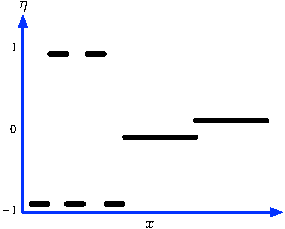
\includegraphics[width=3in]{figs/adaptive-rationale.pdf}
\end{center}
\caption{For values of $x$ on the left half of the shown interval, the
  pointwise bias $\eta(x)$ is close to $-1$ or $1$, and thus a small value of $k$ will yield an accurate prediction. Larger $k$ will not do as well, because they may run into neighboring regions with different labels. For values of $x$ on the right half of the interval, $\eta(x)$ is close to $0$, and thus large $k$ is essential for accurate prediction.}
\label{fig:rationale}
\end{figure}

Our estimator allows us to give rates of convergence that are tighter and more 
transparent than those customarily obtained in nonparametric statistics. Specifically, for any point $x$ in the instance space $\X$, we define a notion of the {\it advantage at $x$}, denoted $\adv(x)$, which is rather like a local margin. We show that the prediction at $x$ is very likely to be correct once the number of training points exceeds~$\tilde{O}(1/\adv(x))$. Universal consistency follows by establishing that almost all points have positive advantage.

{\bf Yoav:} I would add to this figure something to indicate that
points that are far from the boundary converge faster.
  
\subsection{Relation to other work in nonparametric estimation}

For linear separators and many other {\it parametric} families of classifiers, it is possible to give rates of convergence that hold without any assumptions on the input distribution $\mu$ or the conditional expectation function $\eta$. This is not true of nonparametric estimation: although any target function can in principle be captured, the number of samples needed to achieve a specific level of accuracy will inevitably depend upon aspects of this function such as how fast it changes~\cite[chapter 7]{DGL96}. As a result, nonparametric statistical theory has focused on (1) asymptotic consistency, ideally without assumptions, and (2) rates of convergence under a variety of smoothness assumptions.

Asymptotic consistency has been studied in great detail for the $k$-nearest neighbor classifier, when $k$ is allowed to grow with the number of data points $n$. The risk of the classifier, denoted $R_n$, is its error rate on the underlying distribution $P$; this is a random variable that depends upon the set of training points seen. Cover and Hart~\cite{CH67} showed that in general metric spaces, under the assumption that every $x$ in the support of $\mu$ is either a continuity point of $\eta$ or has $\mu(\{x\}) > 0$, the expected risk $\E R_n$ converges to the Bayes-optimal risk $R^*$, as long as $k \rightarrow \infty$ and $k/n \rightarrow 0$. For points in finite-dimensional Euclidean space, a series of results starting with Stone~\cite{S77} established consistency without any assumptions on $\mu$ or $\eta$, and showed that $R_n \rightarrow R^*$ almost surely~\cite{DGKL94}. More recent work has extended these {\it universal consistency} results---that is, consistency without assumptions on $\eta$---to arbitrary metric measure spaces $(\X, d, \mu)$ that satisfy a certain differentiation condition~\cite{CG06,ChaudhuriDasgupta2014}.

Rates of convergence have been obtained for $k$-nearest neighbor classification under various smoothness conditions including Holder conditions on $\eta$~\cite{KP95,G81} and ``Tsybakov margin'' conditions~\cite{MT99,AT07,ChaudhuriDasgupta2014}. Such assumptions have become customary in nonparametric statistics, but they leave a lot to be desired. First, they are uncheckable: it is not possible to empirically determine the smoothness given samples. Second, they view the underlying distribution $P$ through the tiny window of two or three parameters, obscuring almost all the remaining structure of the distribution that also influences the rate of convergence. Finally, because nonparametric estimation is {\it local}, there is the intriguing possibility of getting different rates of convergence in different regions of the input space: a possibility that is immediately defeated by reducing the entire space to two smoothness constants.

The first two of these issues are partially addressed by recent work of \cite{ChaudhuriDasgupta2014}, who analyze the finite sample risk of $k$-NN classification without any assumptions on $P$. Their bounds involve terms that measure the probability mass of the input space in a carefully defined region around the decision boundary, and are shown to be ``instance-optimal'': that is, optimal for the specific distribution $P$, rather than minimax-optimal for some very large class containing $P$. However, the expressions for the risk are somewhat hard to parse, in large part because of the interaction between $n$ and $k$.

In the present paper, we obtain finite-sample rates of convergence that are ``instance-optimal'' not just for the specific distribution $P$ but also for the specific query point. This is achieved by defining a {\it margin}, or {\it advantage}, at every point in the input space, and giving bounds (Theorem~\ref{thm:pointwise-rate}) entirely in terms of this quantity. For parametric classification, it has become common to define a notion of margin that controls generalization. In the nonparametric setting, it makes sense that the margin would in fact be a function $\X \rightarrow \R$, and would yield different generalization error bounds in different regions of space. Our adaptive nearest neighbor classifier allows us to realize this vision in a fairly elementary manner.

\paragraph{Organization.} 
{\new{We begin by formally describing the setup and notation in \Cref{sec:setup}.
Then, a formal description of the adaptive $k$-NN algorithm is given in~\Cref{sec:alg}.
In \Cref{sec:gen1,sec:gen2,sec:gen3} we state and prove consistency and generalization
bounds for this classifier, and compare them with previous bounds in the $k$-NN literature.
These bounds exploit a general VC-based uniform convergence statement
which is presented and proved in a self-contained manner in \Cref{sec:ucecm}.}}


\section{Setup}\label{sec:setup}

Take the instance space to be a separable metric space $(\X, d)$ and the label space to be $\Y = \{\pm 1\}$. All data are assumed to be drawn i.i.d.\ from a fixed unknown distribution $P$ over $\X \times \Y$.

Let $\mu$ denote the marginal distribution on $\X$: if $(X,Y)$ is a 
random draw from $P$, then
$$ \mu(S) = \pr(X \in S)$$
for any measurable set $S \subseteq \X$. For any $x \in \X$, the conditional expectation, or {\em bias}, of $Y$ given $x$, is
$$ \eta(x) = \E(Y| X = x) \in [-1,1] .$$ 
Similarly, for any measurable set $S$ with $\mu(S) > 0$, the
conditional expectation of $Y$ given $X \in S$ is
$$ \eta(S) = \E(Y| X \in S) = \frac{1}{\mu(S)} \int_S \eta(x) \ d \mu(x) .$$

The risk of a classifier $g: \X \rightarrow \{-1,+1,?\}$ is the probability that it is incorrect on pairs $(X,Y) \sim P$,
\begin{equation}
R(g) = P(\{(x,y): g(x) \neq y\}).
\label{eq:risk}
\end{equation}
The Bayes-optimal classifier $g^*$, as given in (\ref{eq:bayes-opt}), depends only on $\eta$, but its risk $R^*$ depends on $\mu$. For a classifier $g_n$ based on $n$ training points from $P$, we will be interested in whether $R(g_n)$ converges to $R^*$, and the rate at which this convergence occurs.

The algorithm and analysis in this paper depend heavily on the probability masses and biases of balls in $\X$. For $x \in \X$ and $r \geq 0$, let $B(x,r)$ denote the closed ball of radius $r$ centered at $x$, 
$$ B(x,r) = \{ z \in \X : d(x,z) \leq r \} .$$
For $0 \leq p \leq 1$, let $r_p(x)$ be the smallest radius $r$ such that $B(x,r)$ has probability mass at least $p$, that is,
\begin{equation}
r_p(x) = \inf \{r \geq 0: \mu(B(x,r)) \geq p \}.
\label{eq:probability-radius}
\end{equation}
It follows that $\mu(B(x,r_p(x))) \geq p$.

The {\it support} of the marginal distribution $\mu$ plays an important role in convergence proofs and is formally defined as
$$ \supp(\mu) = \{x \in \X: \mbox{$\mu(B(x,r)) > 0$ for all $r > 0$}\} .$$
It is a well-known consequence of the separability of $\X$ that $\mu(\supp(\mu)) = 1$~\cite{CH67}.



\section{The adaptive $k$-nearest neighbor algorithm}\label{sec:alg}

The algorithm is given a labeled training set
$(x_1, y_1), \ldots, (x_n, y_n) \in \X \times \Y$.
Based on these points, it is able to compute empirical estimates of the probabilities and biases of different balls.

For any set $S \subseteq \X$, we define its empirical count and probability mass as
\begin{align}
\notag \#_n(S) &= |\{i: x_i \in S\}| \\
\mu_n(S) &= \frac{\#_n(S)}{n} .
\label{eq:empirical-mass}
\end{align}
If this is non-zero, we take the empirical bias to be
\begin{equation}
\eta_n(S) = \frac{\sum_{i: x_i \in S} y_i}{\#_n(S)} .
\label{eq:empirical-bias}
\end{equation}

\begin{figure}
\fbox{\begin{minipage}{5.25in}
\vspace{.1in}
\begin{center}
\begin{minipage}{5in}
Given: 
\begin{itemize}
\item training set $(x_1, y_1), \ldots, (x_n, y_n) \in \X \times \{\pm 1\}$
\item confidence parameter $0 < \delta < 1$
\end{itemize}

\vspace{.1in}
To predict at $x \in \X$:
\begin{itemize}
\item For any integer $k$, let $B_k(x)$ denote the smallest ball centered at $x$ that contains at least $k$ training points.
\item Find the smallest $0 < k \leq n$ for which the $B_k(x)$ has a
  {\em significant bias}: that is,~$\left|\eta_n(B_k(x))\right| > \Delta(n, \#_n(B_k(x)),\delta)$, where
\begin{equation}
\Delta(n,m,\delta) = c_1 \sqrt{\frac{\log n + \log (1/\delta)}{m}}.
\label{eq:delta-default}
\end{equation}
\item If there exists such a ball, return label $\sign(\eta_n(B_k(x)))$.
\item If no such ball exists: return ``?''
\end{itemize}
\vspace{.1in}
\end{minipage}
\end{center}
\end{minipage}}
\caption{The adaptive $k$-NN (AKNN) classifier. The absolute constant $c_1$ is from Lemma~\ref{lemma:bias}.}
\label{fig:alg}
\end{figure}

The adaptive $k$-NN algorithm (AKNN) is shown in Figure~\ref{fig:alg}. It makes a prediction at $x$ by growing a ball around $x$ until the ball has significant bias, and then choosing the corresponding label. In some cases, a ball of sufficient bias may never be obtained, in which event ``?'' is returned. In what follows, let $g_n: \X \rightarrow \{-1,+1,?\}$ denote the AKNN classifier.

Later, we will also discuss a variant of this algorithm in which a modified confidence interval,
\begin{equation}
\Delta(n,m,\delta) = c_1 \sqrt{\frac{d_0 \log n + \log (1/\delta)}{m}},
\label{eq:delta-modified}
\end{equation}
is used, where $d_0$ is the VC dimension of balls in $(\X,d)$. 

\section{Pointwise advantage and rates of convergence}\label{sec:gen1}

We now provide finite-sample rates of convergence for the adaptive nearest neighbor rule. For simplicity, we give convergence rates that are specific to any query point $x$ and that depend on a suitable notion of the ``margin'' of distribution $P$ around $x$.

Pick any $p, \gamma > 0$. Recalling definition (\ref{eq:probability-radius}), we say a point $x \in \X$ is $(p, \gamma)$-salient if either of the following two conditions hold:
\begin{itemize}
\item $\eta(x) > 0$, and $\eta(B(x,r)) > 0$ for all $r \in [0,r_p(x))$, and $\eta(B(x,r_p(x))) \geq \gamma$ \qquad OR
% \end{itemize}
% or
% \begin{itemize}
\item $\eta(x) < 0$, and $\eta(B(x,r)) < 0$ for all $r \in [0,r_p(x))$, and $\eta(B(x,r_p(x))) \leq -\gamma$.
\end{itemize}
A point $x$ can satisfy this definition for a variety of pairs $(p,\gamma)$. The {\it advantage} of $x$ is taken to be the largest value of $p\gamma^2$ over all such pairs:
\begin{equation}
\adv(x) = 
\left\{
\begin{array}{ll}
\sup \{ p \gamma^2: \mbox{$x$ is $(p,\gamma)$-salient}\} & \mbox{if $\eta(x) \neq 0$} \\
0 & \mbox{if $\eta(x) = 0$}
\end{array}
\right.
\label{eq:advantage}
\end{equation}
We will see (Lemma~\ref{lemma:positive-advantage}) that under a mild condition on the underlying metric measure space, almost all $x$ with $\eta(x) \neq 0$ have a positive advantage.

\subsection{Advantage-based finite-sample bounds}

%\begin{theorem}[Pointwise convergence rate]
%There is an absolute constant $C > 0$ for which the following holds. Pick a point $x \in \supp(\mu)$ and a confidence parameter $0 < \delta < 1$. Suppose the AKNN algorithm (Figure~\ref{fig:alg}) is used to define a classifier $g_n$ based on $n$ training points chosen i.i.d.\ from $P$. If the size of the training set satisfies 
%$$ n \geq \frac{C}{\adv(x)} \max \left( \log \frac{1}{\adv(x)}, \ \log \frac{1}{\delta} \right),$$
%then with probability at least $1-\delta$, we will have $g_n(x) = g^*(x)$.
%\label{thm:pointwise-rate}
%\end{theorem}
%\shay{The above formulation confuses me. Specifically, the quantifiers are somewhat vague:
%It seems that $x$ and $\delta$ have the same quantification but, as far as I understand, they do not:
%$x$ is quantified universally whereas $\delta$  is a parameter of the algorithm.
%In other words, first we pick any $\delta\in [0,1]$, which specifies the algorithm,
%and then we argue: for every $\mu$ and for every $x\in \supp(\mu)$, etcetera.
%I suggest to use ``pick'' for $\delta$, and use ``let'' for $x$.
%Here is an alternative formulation (feel free to modify/discard).}

{\new{The following theorem shows that for every point $x$,
if the sample size $n$ satisfies $n\gtrapprox 1/\adv(x)$,
then the label of $x$ is likely to be $g^*(x)$, where $g^*$ is the bayes optimal classifier.}}

\begin{theorem}[Pointwise convergence rate]
There is an absolute constant $C > 0$ for which the following holds.
Let $0 < \delta < 1$ denote the confidence parameter in the AKNN algorithm (\Cref{fig:alg}),
and suppose the algorithm is used to define a classifier $g_n$ based on $n$ training points chosen i.i.d.\ from $P$. 
Then, for every point $x\in\supp(\mu)$, if
\[n \geq \frac{C}{\adv(x)} \max \left( \log \frac{1}{\adv(x)}, \ \log \frac{1}{\delta} \right)\]
then with probability at least $1-\delta$ we have that $g_n(x)=g^*(x)$.
\label{thm:pointwise-rate}
\end{theorem}



{\new{If we further assume that the family of all balls in the space has a finite VC dimension $d_o$ then 
we can strengthen \Cref{thm:pointwise-rate} so that the guarantee holds with high probability \underline{simultaneously} for all $x\in \supp(\mu)$.
This is achieved by a modified version of the algorithm that uses confidence interval (\ref{eq:delta-modified}) instead of (\ref{eq:delta-default}).}}

%\begin{theorem} [Uniform convergence rate]
%Suppose that the set of balls in $(\X,d)$ has finite VC dimension $d_0$, and that the algorithm of Figure~\ref{fig:alg} is used with confidence interval (\ref{eq:delta-modified}) instead of (\ref{eq:delta-default}). Pick any $0 < \delta < 1$. With probability at least $1-\delta$, the resulting classifier $g_n$ will have $g_n(x) = g^*(x)$ for all $x \in \supp(\mu)$ for which 
%$$ n \geq \frac{C}{\adv(x)} \max \left( d_0 \log \frac{d_0}{\adv(x)}, \ \log \frac{1}{\delta} \right).$$
%\label{thm:uniform-rate}
%\end{theorem}

%\shay{Perhaps we should try and state the above two theorems in a similar way
%in order to highlight the (somewhat subtle) difference between them: 
%``for every $x$ w.h.p'' in Theorem 1 versus `w.h.p for every $x$'' in Theorem 2.}

\begin{theorem} [Uniform convergence rate]
%There is an absolute constant $C > 0$ for which the following holds.
%Let $0 < \delta < 1$ denote the confidence parameter in the AKNN algorithm (\Cref{fig:alg}).
Suppose that the set of balls in $(\X,d)$ has finite VC dimension $d_0$, and that the algorithm of Figure~\ref{fig:alg} is used with confidence interval (\ref{eq:delta-modified}) instead of (\ref{eq:delta-default}). 
Then, with probability at least $1-\delta$, the resulting classifier $g_n$ satisfies the following: 
for every point~$x\in\supp(\mu)$, if
\[n \geq \frac{C}{\adv(x)} \max \left( \log \frac{1}{\adv(x)}, \ \log \frac{1}{\delta} \right)\]
then $g_n(x)=g^*(x)$.
\label{thm:uniform-rate}
\end{theorem}


A key step towards proving Theorems~\ref{thm:pointwise-rate} and \ref{thm:uniform-rate} is to identify the subset of $\X$ that is likely to be correctly classified for a given number of training points $n$. This follows the rough outline of \cite{ChaudhuriDasgupta2014}, which gave rates of convergence for $k$-nearest neighbor, but there are two notable differences. First, we will see that the likely-correct sets obtained in that earlier work (for $k$-NN) are subsets of those we obtain for the new adaptive nearest neighbor procedure. Second, the proof for our setting is considerably more streamlined; for instance, there is no need to devise tie-breaking strategies for deciding the identities of the $k$ nearest neighbors.



\subsection{A comparison with $k$-nearest neighbor}
\label{sec:knn-comparison}

For $a \geq 0$, let $\X_a$ denote all points with advantage greater than $a$:
\begin{equation}
\X_a = \{x \in \supp(\mu): \adv(x) > a \} .
\label{eq:advantage-set}
\end{equation}
In particular, $\X_0$ consists of all points with positive advantage. 

By Theorem~\ref{thm:pointwise-rate}, points in $\X_a$ are likely to be correctly classified when the number of training points is~$\widetilde{\Omega}(1/a)$, where the $\widetilde{\Omega}(\cdot)$ notation ignores logarithmic terms.
In contrast, the work of \cite{ChaudhuriDasgupta2014} showed that with $n$ training points, the $k$-NN classifier is likely to correctly classify the following set of points:
\begin{align*}
\X'_{n,k} &= \{x \in \supp(\mu): \eta(x) > 0, \eta(B(x,r)) \geq k^{-1/2} \mbox{\ for all $0 \leq r \leq r_{k/n}(x)$}\} \\
&\ \cup \{x \in \supp(\mu): \eta(x) < 0, \eta(B(x,r)) \leq -k^{-1/2} \mbox{\ for all $0 \leq r \leq r_{k/n}(x)$}\} .
\end{align*}
Such points are $(k/n, k^{-1/2})$-salient and thus have advantage at least $1/n$. In fact,
$$ \bigcup_{1 \leq k \leq n} \X'_{n,k} \subseteq \X_{1/n} .$$
In this formal sense, the adaptive nearest neighbor procedure is able to perform as well as all choices of $k$ simultaneously.

\section{Universal consistency}\label{sec:gen2}
\label{sec:universal-consistency}

In this section we study the convergence of $R(g_n)$ to the Bayes risk $R^*$ as the number of points $n$ grows. An estimator is described as universally consistent in a metric measure space $(\X, d, \mu)$ if it has this desired limiting behavior for all conditional expectation functions $\eta$.

Earlier work~\cite{ChaudhuriDasgupta2014} has established the universal consistency of $k$-nearest neighbor (for $k/n \rightarrow 0$ and $k/(\log n) \rightarrow \infty$) in any metric measure space that satisfies the Lebesgue differentiation condition: that is, for any bounded measurable $f: \X \rightarrow \R$ and for almost all ($\mu$-a.e.) $x \in \X$,
\begin{equation}
\lim_{r \downarrow 0} \frac{1}{\mu(B(x,r))} \int_{B(x,r)} f \ d\mu = f(x) .
\label{eq:lebesgue-condition}
\end{equation}
This is known to hold, for instance, in any finite-dimensional normed space or any doubling metric space~\cite[Chapter 1]{H01}.

We will now see that this same condition implies the universal consistency of the adaptive nearest neighbor rule. To begin with, it implies that almost every point has positive advantage.
\begin{lemma}
Suppose metric measure space $(\X, d, \mu)$ satisfies condition (\ref{eq:lebesgue-condition}). Then,
{\new{for any conditional expectation $\eta$}}, the set of points
$$ \{x \in \X: \eta(x) \neq 0, \, \adv(x) = 0\}$$
has zero $\mu$-measure.
\label{lemma:positive-advantage}
\end{lemma}
\begin{proof}
Let $\X' \subseteq \X$ consist of all points $x \in \supp(\mu)$ for which condition (\ref{eq:lebesgue-condition}) holds true with $f=\eta$, that is, $\lim_{r \downarrow 0} \eta(B(x,r)) = \eta(x)$. 
Since $\mu(\supp(\mu))=1$, it follows that $\mu(\X') = 1$. 

Pick any $x \in \X'$ with $\eta(x) \neq 0$; without loss of generality, $\eta(x) > 0$. By (\ref{eq:lebesgue-condition}), there exists $r_o > 0$ such that
$$\eta(B(x,r)) \geq \eta(x)/2 \mbox{\  for all \ } 0 \leq r \leq r_o.$$
Thus $x$ is $(p,\gamma)$-salient for $p = \mu(B(x,r_o)) > 0$ and $\gamma = \eta(x)/2$, and hence has positive advantage.
\end{proof}

Universal consistency follows as a consequence; the proof details are deferred to Section~\ref{sec:proof-outline}.
\begin{theorem}[Universal consistency]
Suppose the metric measure space $(\X, d, \mu)$ satisfies condition (\ref{eq:lebesgue-condition}). Let $(\delta_n)$ be a sequence in $[0,1]$ with (1) $\lim_{n \rightarrow \infty} \delta_n = 0$, (2) $\lim_{n \rightarrow \infty} (\log (1/\delta_n))/n = 0$, and (3) $\lim_{N \rightarrow \infty} \sum_{n \geq N} \delta_n = 0$. Let the classifier $g_{n, \delta_n}: \X \rightarrow \{-1,+1,?\}$ be the result of applying the adaptive nearest neighbor procedure (Figure~\ref{fig:alg}) with $n$ points chosen i.i.d.\ from $P$ and with confidence parameter $\delta_n$. Letting $R_n = R(g_{n,\delta_n})$ denote the risk of $g_{n,\delta_n}$, we have $R_n \rightarrow R^*$ almost surely.
\label{thm:universal-consistency}
\end{theorem}

\section{Analysis and proofs}\label{sec:gen3}
\label{sec:proof-outline}

The first step in establishing advantage-dependent rates of convergence is to bound the accuracy of empirical estimates of probability mass and bias. This is achieved by a careful choice of large deviation bounds.

\subsection{Large deviation bounds}

Suppose we draw $n$ points $(x_1, y_1), \ldots, (x_n, y_n)$ from $P$. If $n$ is reasonably large, we would expect the empirical mass $\mu_n(S)$ of any set $S \subset \X$, as defined in (\ref{eq:empirical-mass}), to be close to its probability mass under $\mu$. The following lemma, from \cite{ChaudhuriDasgupta2010}, quantifies one particular aspect of this.
\begin{lemma}[\cite{ChaudhuriDasgupta2010}, Lemma 7]
There is a universal constant $c_0$ such that the following holds. Let~$\B$ be any class of measurable subsets of $\X$ of VC dimension $d_0$. Pick any $0 < \delta < 1$. Then with probability at least $1-\delta^2/2$ over the choice of $(x_1, y_1), \ldots, (x_n, y_n)$, for all $B \in \B$ and for any integer $k$, we have
$$ \mu(B) \geq \frac{k}{n} + \frac{c_0}{n} \max \left( k, d_0 \log \frac{n}{\delta} \right)
\ \ \implies \ \ 
\mu_{n}(B) \geq \frac{k}{n} .$$
\label{lemma:points-in-balls}
\end{lemma}

Likewise, we would expect the empirical bias $\eta_n(S)$ of a set $S \subset \X$, as defined in (\ref{eq:empirical-bias}), to be close to its true bias $\eta(S)$. The latter is defined whenever $\mu(S) > 0$.
\begin{lemma}
There is a universal constant $c_1$ for which the following holds. Let $\mathcal{C}$ be a class of subsets of $\X$ with VC dimension $d_0$. Pick any $0 < \delta < 1$. Then with probability at least $1-\delta^2/2$ over the choice of $(x_1, y_1), \ldots, (x_n, y_n)$, for all $C \in \mathcal{C}$,
  $$ \left| \eta_n(C) - \eta(C) \right| \ \leq \ \Delta(n, \#_n(C), \delta) $$
where $\#_n(C) = |\{i: x_i \in B\}|$ is the number of points in $C$ and 
\begin{equation}
\Delta(n,k,\delta) = c_1 \sqrt{\frac{d_0 \log n + \log (1/\delta)}{k}} .
\label{eq:delta-defn}
\end{equation}
\label{lemma:bias}
\end{lemma}

\Cref{lemma:bias} is a special case\footnote{\new{Indeed, \Cref{lemma:bias} follows from \Cref{thm:UCECM} 
by plugging $\cA = \{\X\times\{+1\}, \X\times\{-1\}\}$ and $\B = \{C\times\{\pm 1\} : C\in\mathcal{C}\}$.}} of a uniform convergence bound for conditional probabilities (\Cref{thm:UCECM}) 
that we present and prove in \Cref{sec:ucecm}.

%\shay{TODO: explain somewhere how to derive Lemma 6 from Theorem 10 and give a pointer here to this explanation.}

\subsection{Proof of Theorem~\ref{thm:pointwise-rate}}

\begin{lemma}
There is a universal constant $c_3 > 0$ for which the following holds. Pick any $x \in \supp(\mu)$ with $\adv(x) > 0$. Fix any $0 < \delta < 1$. If the number of training points satisfies
$$ n \geq \frac{c_3}{\adv(x)} \max\left(\log \frac{c_3}{\adv(x)}, \ \log \frac{1}{\delta} \right), $$
then with probability at least $1-\delta^2$ over the choice of training data, the adaptive nearest neighbor rule will have $g_n(x) = g^*(x)$.
\label{lemma:pointwise}
\end{lemma}
\begin{proof}
Define $c_2 = \max(c_1, 1/2) \sqrt{1+c_o}$, where $c_o$ and $c_1$ are the constants from Lemmas~\ref{lemma:points-in-balls} and \ref{lemma:bias}, and take $c_3 = 16 c_2^2$.

Suppose $\eta(x) > 0$; the negative case is symmetric. The set $\B$ of all balls centered at $x$ is easily seen to have VC dimension $d_0 = 1$. By Lemmas~\ref{lemma:points-in-balls} and \ref{lemma:bias}, we have that with probability at least $1-\delta^2$, the following two properties hold for all $B \in \B$:
\begin{enumerate}
\item For any integer $k$, we have $\#_n(B) \geq k$ whenever $n \mu(B) \geq k + c_0 \max(k, \log (n/\delta))$.
\item $|\eta_n(B) - \eta(B)| \leq \Delta(n, \#_n(B), \delta)$.
\end{enumerate}
Assume henceforth that these hold.

By definition of advantage, point $x$ is $(p,\gamma)$-salient for some $p,\gamma> 0$ with $\adv(x) = p\gamma^2$. The lower bound on $n$ implies that
\begin{equation}
\gamma \geq 2c_2 \sqrt{\frac{\log n + \log (1/\delta)}{np}} ,
\label{eq:gamma}
\end{equation}
or equivalently that $n \cdot \adv(x) \geq 4c_2^2 (\log n + \log (1/\delta))$.

Set $k = np/(1 + c_0)$. By (\ref{eq:gamma}) we have $np \geq 4 c_2^2 \log (n/\delta)$ and thus $k \geq \log (n/\delta)$. As a result, $np \geq k + c_0 \max(k, \log (n/\delta))$, and by property 1, the ball $B = B(x, r_p(x))$ has $\#_n(B) \geq k$. This means, in turn, that by property 2,
\begin{align*}
\eta_n(B) &\geq \ \eta(B) - \Delta(n, k, \delta)
= \gamma - c_1 \sqrt{\frac{\log (n/\delta)}{k}} \\
&\geq 2c_2 \sqrt{\frac{\log (n/\delta)}{np}} - c_1 \sqrt{\frac{\log (n/\delta)}{k}}
\geq 2c_1 \sqrt{\frac{\log (n/\delta)}{k}} - c_1 \sqrt{\frac{\log (n/\delta)}{k}} \\
&= c_1 \sqrt{\frac{\log (n/\delta)}{k}} \geq \Delta(n, \#_n(B), \delta) .
\end{align*}
Thus ball $B$ would trigger a prediction of $+1$.

At the same time, for any ball $B' = B(x, r)$ with $r < r_p(x)$,
$$ \eta_n(B') \geq \eta(B') - \Delta(n, \#_n(B'), \delta) > -\Delta(n, \#_n(B'), \delta) $$
and thus no such ball will trigger a prediction of $-1$. Therefore, the prediction at $x$ must be $+1$.
\end{proof}
\subsection{Proof of Theorem~\ref{thm:uniform-rate}}

This proof follows much the same outline as that of Theorem~\ref{thm:pointwise-rate}. A crucial difference is that uniform large deviation bounds (Lemmas~\ref{lemma:points-in-balls} and \ref{lemma:bias}) are applied to the class of all balls in $\X$, which is assumed\footnote{This is motivated by finite-dimensional Euclidean space $\mathbb{R}^{D}$, where it holds with $d_0 = D+1$ (\cite{dudley79}).} to have finite VC dimension $d_0$. In contrast, the proof of Theorem~\ref{thm:pointwise-rate} only applies these bounds to the class of balls centered at a specific point, which has VC dimension at most 1 in any metric space.

%\sanjoy{How much more do we need to say here? There is more detail in the appendix.}



\subsection{Proof of Theorem~\ref{thm:universal-consistency}}

Recall from (\ref{eq:advantage-set}) that $\X_a$ denotes the set of points with advantage $> a$.
\begin{lemma}
Pick any $0 < \delta < 1$ as a confidence parameter for the AKNN estimator of Figure~\ref{fig:alg}. Fix any $a > 0$. If the number of training points $n$ satisfies
$$ n \geq \frac{c_3}{a} \max\left(\log \frac{c_3}{a}, \ \log \frac{1}{\delta} \right), $$
then with probability at least $1-\delta$, the resulting classifier $g_n$ has risk
$$ R(g_n) - R^* \leq \delta + \mu(\X_0 \setminus \X_a) .$$
\label{lemma:advantage-set-convergence}
\end{lemma}
\begin{proof}
From Lemma~\ref{lemma:pointwise}, we have that for any $x \in \X_a$, 
$$ \pr_n(g_n(x) \neq g^*(x)) \leq \delta^2 ,$$
where $\pr_n$ denotes probability over the choice of training points. Thus, for $X \sim \mu$,
$$ \E_n \E_X 1(g_n(X) \neq g^*(X) | X \in \X_a) \leq \delta^2 ,$$
and by Markov's inequality,
$$ \pr_n [\pr_X (g_n(X) \neq g^*(X) |  X \in \X_a) \geq \delta] \leq \delta.$$
Thus, with probability at least $1-\delta$ over the training set,
$$\pr_X (g_n(X) \neq g^*(X) |  X \in \X_a) \leq \delta .$$
On points with $\eta(x) = 0$, both $g_n$ and the Bayes-optimal $g^*$ incur the same risk. Thus
\begin{align*}
R(g_n) - R^*
&\leq \pr_X(g_n(X) \neq g^*(X) | X \in \X_a) + \pr_X(X \not\in \X_a, \eta(X) \neq 0) \\ 
&\leq \delta + \pr_X(X \in \X_0 \setminus \X_a) + \pr_X(\adv(X) = 0, \eta(X) \neq 0) \\ 
&\leq \delta + \mu(\X_0 \setminus \X_a),
\end{align*}
where we invoke Lemma~\ref{lemma:positive-advantage} for the last step.
\end{proof}

We now complete the proof of Theorem~\ref{thm:universal-consistency}. Given the sequence of confidence parameters $(\delta_n)$, define a sequence of advantage values $(a_n)$ by
$$ a_n = \frac{c_3}{n} \max \left( 2 \log n, \ \log \frac{1}{\delta_n} \right) .$$
The conditions on $(\delta_n)$ imply $a_n \rightarrow 0$.

Pick any $\epsilon > 0$. By the conditions on $(\delta_n)$, we can pick $N$ so that $\sum_{n \geq N} \delta_n \leq \epsilon$. Let $\omega$ denote a realization of an infinite training sequence $(X_1, Y_1), (X_2, Y_2), \ldots$ from $P$. By Lemma~\ref{lemma:advantage-set-convergence}, for any positive integer $N$,
$$ \pr \left(\omega: \exists n \geq N \mbox{\ s.t.\ } R(g_n(\omega)) - R^* > \delta_n + \mu(\X_0 \setminus \X_{a_n}) \right) \leq \sum_{n \geq N} \delta_n \leq \epsilon.$$
Thus, with probability at least $1-\epsilon$ over the training sequence $\omega$, we have that for all $n \geq N$,
$$ R(g_n(\omega)) - R^* \leq \delta_n + \mu(\X_0 \setminus \X_{a_n}) ,$$
whereupon $R(g_n(\omega)) \rightarrow R^*$ (since $\delta_n, a_n \rightarrow 0$ and $\lim_{a \downarrow 0} \mu(\X_0 \setminus \X_a) = 0$). Since this holds for any $\epsilon  >0$, the theorem follows.


\section{Uniform Convergence of Empirical Conditional Measures}
\label{sec:ucecm}

\subsection{Formal Statement}

Let $P$ be a distribution over $X$, and let $\cA,\cB$ be two collections of events.
Consider $n$ independent samples from~$P$, denoted by~$x_1,\ldots,x_n$.
We would like to estimate $P(A \vert B)$ simultaneously for all~$A\in\cA, B\in \cB$.
It is natural to consider the empirical estimates:
\[P_n(A\vert B)=\frac{\sum_i 1_{[x_i\in A \cap B]}}{\sum_i 1_{[x_i\in B]}}.\]
We study when (and to what extent) these estimates provide a good approximation.
Note that the case where $\cB=\{X\}$ (i.e., in which one estimates $P(A)$
using $P_n(A)$ simultaneously for all $A\in\cA$) is handled by the classical VC theory.
Throughout this section we assume that both $\cA,\cB$ have a finite VC-dimension, 
and we let $d_0$ denote an upper bound on both $\mathsf{VC}(\cA)$ and $\mathsf{VC}(\cB)$.

To demonstrate the kinds of statements we would like to derive,
consider the case where each of~$\cA,\cB$ contains only one event:
$\cA=\{A\}$, and $\cB=\{B\}$,
and set $k(B)=\sum_i 1_{[x_i\in B]}$.
A Chernoff bound implies that conditioned on the event that $k(B)>0$, 
the following holds with probability at least~$1-\delta$:
\begin{equation}\label{eq:chernoff}
\left\lvert P(A\vert B) - P_n(A \vert B) \right\rvert \leq \sqrt{\frac{2\log(1/\delta)}{k(B)}}.
\end{equation}
To derive it, use that conditioned on $x_i\in B$, the event $x_i\in A$ has probability $P(A\vert B)$, 
and therefore the random variable ``$k(B)\cdot p_n(A \vert B)$'' has a binomial distribution with parameters $k(B)$ and $P(A\vert B)$.

Note that the bound on the error in \Cref{eq:chernoff} depends on $k(B)$ and therefore is data-dependent.
We stress that this is the type of statement we want:
the more samples belong to $B$, the more certain we are with the empirical estimate.
Thus, we would want to prove a statement as follows:

With probability at least~$1-\delta$,
\[\left(\forall A\in\cA\right)\left(\forall B\in\B\right):\left\lvert P(A \vert B) - P_n(A \vert B) \right\rvert \leq O\left(\sqrt{\frac{d_0 \log(1/\delta)}{k(B)}}\right),\]
where $k(B) = \sum_{i=1}^n 1[x_i\in B]$.

The above statement is, unfortunately, false. 
As an example, consider the probability space defined by drawing $x \sim[n]$ uniformly,
and then coloring $x$ by $c_x\in\{\pm 1\}$ uniformly.
For each $i$ let $B_i$ denote the event that~$i$ was drawn,
and let $A$ denote the event that the drawn color was  $+1$.
(formally, $B_i = \{i\}\times\{\pm 1\}$, and $A=[n]\times\{+1\}$).
One can verify that the VC dimension of $\B=\{B_i : i\leq n\}$ and of $\cA=\{A\}$ is at most $1$.
The above statement fails in this setting:
indeed, one can verify that if we draw $n$ samples from this space 
then with a constant probability there will be some  $j$
such that: 
\begin{itemize}
\item[(i)] $j$ always gets the same color (say $+1$), and 
\item[(ii)] $j$ is sampled at least $\Omega(\log n/\log\log n)$ times\footnote{{This follows from analyzing the maximal bin
in a uniform assignment of $\Theta(n)$ balls into $n$ bins~\cite{bins}}}.
\end{itemize}
Therefore, with constant probability we get that 
\[P_n(A\vert B_i) = 1, P(A\vert B_i)=1/2,\]
and so the difference between the error is clearly $1-(1/2)=1/2$,
which is clearly not upper bounded by $O(\sqrt{\log\log n/\log n})$.

We prove the following (slightly weaker) variant:
\begin{theorem}[UCECM]\label{thm:UCECM}
Let $P$ be a probability distribution over $X$, and let $\cA,\cB$
be two families of measurable subsets of $X$ such that $\mathsf{VC}(\cA),\mathsf{VC}(\cB)\leq d_0$.
Let $n\in\mathbb{N}$, and let $x_1\ldots x_n$ be $n$ i.i.d samples from $P$.
The, the following event occurs with probability at least $1-\delta$:
\[\left(\forall A\in\cA\right)\left(\forall B\in\B\right):\left\lvert P(A \vert B) - P_n(A \vert B) \right\rvert \leq 
\sqrt{\frac{k_o}{k(B)}},\]
where $k_o = 1000 \left(d_0 \log(8n) + \log(4/\delta)\right)$, and\footnote{Note that the above inequality makes sense also when $k(B)=0$,
by identifying $\frac{\cdot}{0}$ as $\infty$, and using the convention that $\infty-\infty=\infty$ and that $\infty\leq \infty$.} $k(B) = \sum_{i=1}^n 1[x_i\in B]$.
\end{theorem}

\paragraph{Discussion.}
\Cref{thm:UCECM} can be combined with \Cref{lemma:points-in-balls}
to yield a bound on the minimal $n$ for which $P_n(A \vert B)$ 
is a non-trivial approximation of $P(A \vert B)$.
Indeed, \Cref{lemma:points-in-balls} implies that 
if $n$ is large enough so that $P(B)=\Omega\left(\frac{d_0\log n}{n}\right)$, 
then the empirical estimate $P_n(A\vert B)$ is a decent approximation.
In the context of the adaptive nearest neighbor classifier, this means that the empirical
biases provide meaningful estimates of the true biases for balls whose measure is $\tilde\Omega\left(\frac{d_0}{n}\right)$.
This resembles the learning rate in realizable settings.
%(as explained below, this $n$ is some $\tilde O\left(1/p(B)\right)$).
%
%\Cref{thm:UCECM} can be combined with the following uniform convergence 
%variant to yield a bound on the minimal $n$ for which $p_n(A \vert B)$ 
%is a non-trivial approximation of $p(A \vert B)$
%(as explained below, this $n$ is some $\tilde O\left(1/p(B)\right)$).
%\shay{Is the following lemma is essentially equivalent to \Cref{lemma:points-in-balls}?}
%\begin{lemma}\label{lem:uconeside}
%Set $k_0$ like in \Cref{thm:UCECM}. Then with probability at least $1-\delta$:
%\[
%(\forall B\in \B):~ k(B) \geq \frac{1}{4}np(B) - {k_0}.
%\]
%\end{lemma}
%This implies that if $n$ is large enough so that $p(B)=\tilde\Omega(k/n)=\tilde\Omega\left(\frac{d_0}{n}\right)$
%then the empirical estimate $p_n(A\vert B)$ provides a decent approximation.
%In the context of the adaptive nearest neighbor classifier, this means that the empirical
%biases provide meaningful estimates of the true biases 
%for specialists whose measure is $\tilde\Omega\left(\frac{d_0}{n}\right)$.
%Note the resemblance with the learning rate in realizable settings.
%
%indeed, it implies that roughly $p(B)\pm \sqrt{d/n}$ 
%empirical points from the sample are will indeed belong to $B$
%(with high probability), and so, once $n$ is sufficiently large,
%one can replace the radius of the confidence interval by 
%$\Theta\left(\sqrt{\frac{d\log n}{p(B)n - \sqrt{dn}}}\right)$, 
%which is for a large $n$ roughly $\sqrt{\frac{d\log n}{p(B)n}}$.

We remark that a weaker statement than \Cref{thm:UCECM}
can be derived as a corollary of the classical uniform convergence
result~\citep{vapnik1971uniform}. 
Indeed, since the VC dimension of $\{B\cap A : i\in \I\}$ is at most $d_0$, it follows that 
\[P_n(A\vert B)\approx\frac{P(A\cap B) \pm \sqrt{d_0 / n}}{P(B)\pm \sqrt{d_0 / n}}.\]
However, this bound guarantees non-trivial estimates only once $P(B)$ is roughly $\sqrt{d_0  / n}$.
This is similar to the learning rate in agnostic (i.e., non-realizable) settings.

Another major advantage of the uniform convergence bound in \Cref{thm:UCECM} is that it is data-dependent: 
if many points from the sample belong to $B\in \cB$ (i.e.\ $k(B)$ is large), 
then we get better guarantees on the approximation of $P(A\vert B)$ by $P_n(A\vert B)$ for all $A\in\cA$.



\subsection{Proof of \Cref{thm:UCECM}}

As noted above,
the standard uniform convergence bound for VC classes
can not yield the bound in \Cref{thm:UCECM}.
Instead, we use a variant of it due to~\cite{BBL05} which concerns {\it relative deviations}
(see~\cite{BBL05}: Theorem 5.1 and the discussion before Corollary 5.2).
In order to state the theorem, we need the following notation:
Let $\cC$ be a family of subsets of $\X$. We denote by $\mathbb{S}_\cC:\mathbb{N}\to\mathbb{N}$ the {\it growth function} of $\cC$, which is defined by:
\[
\mathbb{S}_\cC(n) = \max\{\lvert \cC|_R\rvert : R\subseteq X, \lvert R\rvert=n\},
\]
where $\cC|_R=\{C\cap R : C\in\cC\}$ is the projection of $\cC$ to $R$.
\begin{theorem}[\cite{BBL05}]\label{thm:ucrel}
Let $\cC$ be a family of subsets of $\X$  and let $P$
be a distribution over $\X$. Then, the following holds with probability $1-\delta$:
\[
(\forall C\in \cC): \lvert P(C)- P_n(C) \rvert \leq  2\sqrt{P_n(C)\frac{\log\mathbb{S}_\cC(2n) + \log(4/\delta)}{n}} + 4\frac{\log\mathbb{S}_\cC(2n) + \log(4/\delta)}{n}. 
\]
\end{theorem}

Set $\cC = \cB\cup \{A\cap B : A\in\cA, B\in\B\}$. 
We prove \Cref{thm:UCECM} by applying \Cref{thm:ucrel} on $\cC$;
to this end we first upper bound $\mathbb{S}_\cC(n)$.
Let $\mathcal{D}= \{A\cap B :A\in\cA, B\in\cB\}$, so that $\cC = \cB \cup \mathcal{D}$. Then:
\begin{align*}
\mathbb{S}_\cC(n) 
\leq \mathbb{S}_\cB(n) + \mathbb{S}_{\mathcal{D}}(n) \leq \mathbb{S}_\cB(n)  +  \mathbb{S}_\cA(n)\mathbb{S}_\cB(n)\leq 2\mathbb{S}_\cA(n)\mathbb{S}_\cB(n)\leq 2{n \choose \leq d_0}^2\leq 2 (2n)^{2d_0},
\end{align*}
where the second inequality follows since $\mathbb{S}_{\mathcal{D}}(n) \leq \mathbb{S}_\cA(n)\mathbb{S}_\cB(n)$,
the second to last inequality follows from the Sauer-Shelah-Perles Lemma, and the last inequality
follows since~${a \choose \leq b} \leq (2a)^b$.
%\[
%\log\Bigl(2{2n \choose \leq d_0}^2\Bigr) \leq \log \bigl(2{\bigl(4n\bigr)^{2d_0}}\bigr)\leq 2d_0\log \bigl(2{\bigl(4n\bigr)}\bigr)
%\leq 2d_0\log(8n)
%\]
Therefore, applying \Cref{thm:ucrel} on $\cC$ yields that with probability $1-\delta$ the following event holds:
\begin{equation}\label{eq:BBL}
(\forall C\in \cC): \lvert P(C)- P_n(C) \rvert \leq  4\sqrt{P_n(C)\frac{d_0\log 8n + \log(4/\delta)}{n}} + 8\frac{d_0\log 8n + \log(4/\delta)}{n}. 
\end{equation}
For the remainder of the proof we assume that the event in \Cref{eq:BBL} holds and argue that it implies
the conclusion in \Cref{thm:UCECM}.
Let $A\in\cA, B\in\cB$,  
and let $k=n\cdot P_n(B)$ denote the number of data points in $B$. 
We want to show that
\begin{equation}\label{eq:qed}
\left\lvert P(A \vert B) - P_n(A \vert B) \right\rvert \leq 
\sqrt{\frac{k_o}{k}},
\end{equation}
where $k_o=1000 \left(d_0 \log(8n) + \log(4/\delta)\right)$.
Let $j=k\cdot P_n(A\vert B)$ denote the number of data points in~$A\cap B$.
We establish \Cref{eq:qed} by showing that 
\[P(A \vert B) \leq  P_n(A\vert B)  + \sqrt{\frac{k_o}{k}}
~~~\text{ and }~~~ P(A \vert B) \geq  P_n(A\vert B)  - \sqrt{\frac{k_o}{k}}.
\]
In the following calculation it will be convenient to denote $D:=d_0 \log(8n) + \log(4/\delta)$. 
By \Cref{eq:BBL} we get:
\begin{align*}
P(A \vert B) &= \frac{P(A\cap B)}{P(B)}\\
			 &\leq \frac{P_n(A\cap B) + 4\sqrt{P_n(A\cap B)\frac{D}{n}} + 8\frac{D}{n}}{P_n(B) - 4\sqrt{P_n(B)\frac{D}{n}} - 8\frac{D}{n}}\\
			 &=\frac{\frac{P_n(A\cap B)}{P_n(B)} + 4\sqrt{\frac{P_n(A\cap B)}{P_n(B)}\frac{D}{nP_n(B)}} + 8\frac{D}{nP_n(B)}}{1 - 4\sqrt{\frac{D}{nP_n(B)}} - 8\frac{D}{nP_n(B)}}s
%			 &=\frac{P_n(A \vert B) + 4\sqrt{P_n(A \vert B)\frac{d_0\log 8n + \log(4/\delta)}{k}} + 8\frac{d_0\log 8n + \log(4/\delta)}{k}}{1 - 4\sqrt{\frac{d_0\log 8n + \log(4/\delta)}{k}} - 8\frac{d_0\log 8n + \log(4/\delta)}{k}}\\
			 =P_n(A \vert B)\frac{1+ 4\sqrt{\frac{D}{j}} + 8\frac{D}{j}}{1 - 4\sqrt{\frac{D}{k}} - 8\frac{D}{k}},
\end{align*}
where the first inequality follows from \Cref{eq:BBL} and the following equalities are trivial.
Thus,
\begin{equation}\label{eq:16}
P(A \vert B) \leq\frac{j}{k}\Biggl(\frac{1+ 4\sqrt{\frac{D}{j}} + 8\frac{D}{j}}{1 - 4\sqrt{\frac{D}{k}} - 8\frac{D}{k}}\Biggr).
\end{equation}
Next, note that we may assume that $k\geq k_o=1000D$, as otherwise \Cref{eq:qed} trivially holds. Therefore,
\begin{align*}
\frac{1}{1 - 4\sqrt{\frac{D}{k}} - 8\frac{D}{k}} \leq 
1 + 8\sqrt{\frac{D}{k}} + 16\frac{D}{k}. \tag{$(\forall x<\frac{1}{2}):\frac{1}{1-x} \leq 1+2x$}
\end{align*}
Plugging this in \Cref{eq:16}, and using first that $j\leq k$ and then that $1000D\leq k$, yields:
\begin{align*}
P(A \vert B) &\leq \frac{j}{k}\Bigl(1+ 4\sqrt{\frac{D}{j}} + 8\frac{D}{j}\Bigr)\Bigl(1 + 8\sqrt{\frac{D}{k}} + 16\frac{D}{k}\Bigr) \\
&= \frac{j}{k} + 8 \frac{j}{k} \sqrt{\frac{D}{k}} \left( 1 + 2 \sqrt{\frac{D}{k}} \right) + \Bigl( \frac{4\sqrt{j D} + 8D}{k}\Bigr) \Bigl(1 + 4\sqrt{\frac{D}{k}} \Bigr)^2 \\
&\leq \frac{j}{k} + 8 \sqrt{\frac{D}{k}} \left( 1 + 2 \sqrt{\frac{D}{k}} \right) + \Bigl( 4 \sqrt{\frac{D}{k}} + \frac{8D}{k}\Bigr) \Bigl(1 + 4\sqrt{\frac{D}{k}} \Bigr)^2 \\
&\leq \frac{j}{k} + 30\sqrt{\frac{D}{k}} = P_n(A\vert B)  + \sqrt{\frac{k_o}{k}},
\end{align*}
and so 
\[
P(A \vert B) \leq  P_n(A\vert B)  + \sqrt{\frac{k_o}{k}}.
\]
A symmetric argument yields similarly to \Cref{eq:16} that:
\begin{align*}
P(A \vert B) \geq\frac{j}{k}\Biggl(\frac{1 - 4\sqrt{\frac{D}{j}} - 8\frac{D}{j}}{1 + 4\sqrt{\frac{D}{k}} + 8\frac{D}{k}}\Biggr).
\end{align*}
Then, a similar calculation (using the relation $(\forall x > 0):\frac{1}{1+x} \geq 1-2x$) implies that
%\[
%P(A \vert B) \leq \frac{j}{k}\Bigl(1- 4\sqrt{\frac{D}{j}} - 8\frac{D}{j}\Bigr)\Bigl(1 - 4\sqrt{\frac{D}{k}} - 8\frac{D}{k}\Bigr)
%\leq \frac{j}{k} - 30\sqrt{\frac{D}{k}} = P_n(A\vert B)  + \sqrt{\frac{k_o}{k}},
%\]
\[
P(A \vert B) \geq  P_n(A\vert B)  - \sqrt{\frac{k_o}{k}},
\]
which finishes the proof.
\qed






%
%\subsubsection{Overview}
%The idea is to follow the standard argument due to~\cite{vapnik} 
%which derives the standard uniform convergence result (and to modify it accordingly). 
%We follow the exposition of~\cite{anthony}:
%consider a double-sample of size $2n$ from~$p$, denoted by $x_1,\ldots,x_{2n}$.
%Let $S_1$ denote the first half of the sample and $S_2$ the second.
%Define $E_1$ to be the event whose probability we want to bound:
%\[E_1 = \left\{ S_1\in X^n : (\exists B\in \B):~ 
%\left\lvert p(A \vert B) - p_{n,1}(A \vert B) \right\rvert > 
%\sqrt{\frac{k_0}{k_{1}(B)}} \right\},\]
%where $p_{n,1}$ is the empirical measure induced by $S_1$, 
%and $k_{1}(B)=\sum_{i=1}^n 1[x_i\in B]$ ($p_{n,2}, k_{2}$ are defined similarly).
%Let $E_2$ denote the event
%\[E_2 = 
%\left\{
%S_1S_2\in X^{2n} : (\exists B\in\B):~
%\left\lvert p_{n,1}(A \vert B)   -  p_{n,2}(A \vert B) \right\rvert >  
%{\frac{1}{2}}\sqrt{\frac{k_0}{k(B)}}
%\right\},
%\]
%where $k(B) = k_{1}(B)+k_{2}(B)$.
%The strategy is showing that $\Pr[E_1]$ is small by reducing it to showing that $\Pr[E_2]$ 
%is small, and then to show that the latter is small using a standard \emph{symmetrization} argument. 
%For the first part, we would like to argue like in~\cite{anthony}, that
%\begin{equation}\label{eq:anthony} 
%(\forall S_1\in E_1): \Pr_{S_2}[S_1S_2\in E_2]\geq \frac{1}{100}.
%\end{equation}
%Indeed, since $S_1,S_2$ are independent, this implies that $\Pr[E_2 \vert E_1]\geq\frac{1}{100}$ 
%	and therefore that 
%	\[\Pr[E_1] = \frac{\Pr[E_2\land E_1]}{\Pr[E_2 \vert E_1]}\leq 100\Pr[E_1\land E_2] \leq 100\Pr[E_2],\] 
%	which yields the reduction.
%
%However, \Cref{eq:anthony} does not necessarily hold: indeed assume that $\B=\{B\}$ contains
%	a single set $B$ such that $p(B) \ll \frac{1}{n}$ is tiny and $p(A \vert B) = \frac{1}{2}$. 
%	Now, let $S_1\in E_1$, thus
%	\[
%	\left\lvert p(A \vert B) - p_{n,1}(A \vert B) \right\rvert > 
%	\sqrt{\frac{k_0}{k_{1}(B)}}.
%	\]<
%	Now, since $p(B) \ll \frac{1}{n}$ then $B\cap S_2 = \emptyset$ with high probability.
%	This means that $p_{n,2}(\cdot \vert B)$ is undefined and in particular that $S_1S_2\notin E_2$ 
%	with high probability over the choice of $S_2$.
%
%%
%%However, \Cref{eq:anthony} does not necessarily hold: indeed consider
%%	$S_1\in E_1$ such that there is a single $B$ for which 
%%\[
%%\left\lvert p(A \vert B) - p_{n,1}(A \vert B) \right\rvert > 
%%\sqrt{\frac{k_0}{k_{1}(B)}}
%%\]
%%and further assume that 
%%\begin{itemize}
%%\item[(i)] $B$ has a tiny measure, say $p(B) \leq 1/n$,
%%\item[(ii)] $p(A\vert B)= 1/2$, and
%%\item[(iii)] $p_{n,1}(A\vert B) = 0$.
%%\end{itemize}
%%Therefore, $k_2(B)=1$ with a constant probability (at least $1/4$)
%%and so $p_{n,2}(A \vert B)=p_{n,1}(A \vert B)$ 
%%with probability at least~$\frac{1}{8}$ (which implies in particular that ).
%
%To get around this, we introduce an auxiliary event $F$, defined by
%\[F = \left\{S_1\in X^{n} : (\forall B\in\B): p_{n,1}(B) \geq \frac{k_0}{n} \implies p(B)\geq \frac{p_{n,1}(B)}{4}\right\}. \]
%Note that $F$ discards the problematic example from above 
%(by constraining every $B$ that witnesses $E_1$ to have a large probability). 
%The following lemma, which can be seen as a converse to the \Cref{lemma:points-in-balls}, 
%shows that $F$ is a typical event (i.e.\ has a large probability):
%\shay{Maybe move this lemma to after \Cref{lemma:points-in-balls}}
%\begin{lemma}\label{lem:Fistypical}
%Let $\B$ be any class of measurable subsets of $\X$ of VC dimension $d_0$. Pick any $0 < \delta < 1$. Then with probability at least $1-\delta/2$ over the choice of $(x^{(1)}, y^{(1)}), \ldots, (x^{(n)}, y^{(n)})$, for all $B \in \B$ and for any integer $k$, we have
%\[ \mu_n(B) \geq \frac{k_0}{n}
%\ \ \implies \ \ 
%p(B) \geq \frac{\mu_n(B)}{4},\]
%where $k_0 = 200 \left(d_0 \log(3n) + \log(1/\delta)\right)$.
%\end{lemma}
%
%\Cref{lem:Fistypical} allows us to replace \Cref{eq:anthony} with the following:
%\begin{lemma}\label{lem:reduction}
%If $\Pr[E_1]\geq \delta$ then 
%\begin{enumerate}
%\item $\Pr[E_1\cap F] \geq \frac{1}{2}\Pr[E_1]$, and
%\item $(\forall S_1\in E_1\cap F): \Pr_{S_2}[S_1S_2\in E_2] \geq \frac{1}{8}$. 
%\end{enumerate}
%\end{lemma}
%We defer the proof of \Cref{lem:reduction} to a later section, 
%and assume it for now towards proving \Cref{thm:UCECM}.
%
%\Cref{lem:reduction} yields the following win-win situation:
%either $\Pr[E_1] \leq \delta$ and we are done, or:
%\[\frac{\Pr[E_2]}{\Pr[E_1]} \geq  \frac{\Pr[E_2]}{2\Pr[E_1\cap F]} \geq \frac{\Pr[E_2 \vert E_1\cap F]}{2} \geq \frac{1}{16}
%\implies  \Pr[E_1]\leq 16\Pr[E_2],\]
%where the first inequality uses the first item of \Cref{lem:reduction}, 
%the second inequality follows by definition of conditional probability,
%and the last inequality is implied by the the second item of \Cref{lem:reduction}.
%
%
%We proceed to the standard symmetrization argument
%that establishes $\Pr[E_2]\leq\delta/16$. 
%Instead of sampling $S_1S_2\sim p^{2n}$,
%consider the following equivalent process:
%\begin{itemize}
%\item[(i)] Sample $S\sim p^{2n}$.
%\item[(ii)] Partition $S$ uniformly into two subsamples $S_1,S_2$, each of size $n$.
%\end{itemize}
%The following lemma implies that $\Pr[E_2]\leq \delta/16$, and finishes the proof.
%\begin{lemma}\label{lem:e2}
%For every $S\in X^{2n}$
%\[\Pr_{S\to S_1S_2}\left[S_1S_2\in E_2\right]\leq \frac{\delta}{16},\]
%where the randomness is over the uniform partitioning
%of $S$ into $S_1,S_2$.
%\end{lemma}
%\qed
%
%\subsubsection{Proof of \Cref{lem:Fistypical}}
%\Cref{lem:Fistypical} follows from the standard uniform convergence bound with
%the difference of using the multiplicative Chernoff bound instead
%of the additive bound:
%consider a double sample $S=(\samp_1,\samp_2)\sim p^{2n}$.
%Let~$F_1 = \bar F$ denote the event whose probability we want to bound:
%\[
%F_1 =\left\{ S_1\in X^n : (\exists {B\in\B}):
%  p_{n,1}(B) \geq \frac{k_0}{n} \mbox{ and } p(B) < \frac{p_{n,1}(B)}{4}\right\}, 
%\]
%and let $F_2$ denote the event:
%\[
%F_2 = 
%\left\{ S_1S_2\in X^{2n} : (\exists {B\in\B}):
%  p_{n,1}(B) \geq \frac{k_0}{n} \mbox{ and } p_{n,2}(B) < \frac{p_{n,1}(B)}{2}\right\}.
%\]
%The proof is an immediate consequence of the next two lemmas:
%\begin{lemma}\label{lem:aux11}
%$\Pr[F_1]\leq 10\Pr[F_2].$
%\end{lemma}
%\begin{lemma}\label{lem:aux12}
%$\Pr[F_2]\leq \delta/20.$
%\end{lemma}
%\begin{proof}[Proof of Lemma~\ref{lem:aux11}]
%It suffices to show that $\Pr[F_2 \vert F_1]\geq 1/10$.
%	Indeed, this would imply that $\Pr[F_1] \leq 10\Pr[F_1 \cap F_2]\leq 10\Pr[F_2]$.
%	Since $S_2$ and $S_1$ are independent it suffices to show that for all $S_1\in F_1$:
%	\[\Pr_{S_2\sim p^n}\left[(S_1,S_2)\in F_2\right] \geq 1/10.\]
%	Let $S_1\in F_1$, and let $B\in\B$ such that $p_{n,1}(B)\geq\frac{k_0}{n}$ and $p(B)\leq \frac{p_{n,1}(B)}{4}$.
%	We show that $p_{n,2}(B)\leq \frac{p_{n,1}(B)}{2}$ with probability at least~$\frac{1}{10}$.
%	Case (i): if $p(B) < 1/2n$ then 
%\[
%\Pr\left[ p_{n,2}(B) > \frac{p_{n,1}(B)}{2}\right]=\Pr\left[ k_{2}(B) > \frac{k_{1}(B)}{2}\right]
%\leq
%\Pr\left[ k_{2}(B) > 0 \right]
%\leq np(B) < 1/2 < 9/10.
%\]
%Case (ii): else, if $p(B) \geq 1/2n$, 
%	then by the multiplicative\footnote{We use here the following version: if $X=\sum_i X_i$, where the $X_i$'s are independent 0/1 random variables and $\beta\geq 1$ then $\Pr[X\geq (1+\beta)\mu] \leq \exp(\frac{-\beta^2}{2+\beta}\mu)$, where $\mu=\Ex[X]$ (see for example \cite{}).}:
%\[
%\Pr\left[ k_{2}(B) > \frac{k_{1}(B)}{2}\right]
%\leq
%\Pr\left[ k_{2}(B) > 2p(B)\cdot n\right]
%\leq
%\exp\left( \frac{-p(B)\cdot n}{3}\right)\leq \exp(-1/6)\leq 9/10.
%\]
%
%So, conditioned on $F_1$, 
%the event $F_2$ occurs with probability at least $1/10$.
%\end{proof}
%
%\begin{proof}[Proof of Lemma~\ref{lem:aux12}]
%We use a symmetrization argument: instead of sampling $\samp_1$ and then $\samp_2$,
%	first sample $\samp=\samp_1\cup \samp_2$ and then partition it into two equal parts 
%	$\samp_1$ and $\samp_2$ uniformly at random.
%	Now, for a fixed $\samp$ what is the probability (over the random partition) that $F_2$ occurs?
%	Let $\B|_{\samp} = \{B|_{\samp} : B\in\B\}$.
%	It suffices to show that the event
%\[F_2|_{\samp} = 
%\left\{ \{S_1,S_2\}:
%\exists {B\in\B|_{\samp}}:
%  p_{1}(B)\geq \frac{k_0}{n} \mbox{ and } p_{2}(B) < \frac{p_{1}(B)}{2}
%  \right\}
%\]
%has probability at most $\delta/10$ over the partition of $\samp$ into $\samp_1,\samp_2$.
%To this end we use a union bound. 
%	We only need to consider $B$'s in $\B|_{\samp}$ such that $k(B) > k_0$, where $k(B) = k_{1}(B)+ k_{2}(B)$. 
%	Fix such a $B$; without loss of generality assume that the first $k(B)$ points 
%	out of the~$2n$ points in $S$ are in $B$. 	For every $i\leq k(B)$, let $X_i$ denote 
%	the indicator of the event that the $i$'th point in $S$ was drawn into $S_2$.
%	Set~$X=\sum_{i=1}^{k(B)}X_i$.
%	Note that $B$ causes $F_2|_{\samp}$ to occur if and only if $X\leq \frac{k(B)}{3}$.
%	We would like to use a Chernoff bound to bound the probability of this event; 
%	however this bound does not directly apply here as the $X_i$'s are not independent:
%	indeed $S_2$ is generated via a sampling of $n$ points {\it without replacements} from $S$.
%	Nevertheless, Hoeffding (\cite{H63}, Section 6) established\footnote{Theorem 4 in \cite{H63} shows 
%	that any tail bound which is based on the moment-generating function (such as Chernoff bounds) applies to sampling-without-		replacement. \shay{Perhaps move this discussion to a section dedicated to tehcnical background.}} that Chernoff bounds apply also in this setting. Therefore:
%%	and therefore
%%	To analyze this event define a random variable $Y=\sum_{i=1}^{k(B)}Y_i$,
%%	where the $Y_i$'s are independent Bernoulli random variables with probability $1/2$. 
%%	Its moment-generating function upper-bounds that of $X$, i.e. $\evp{\exp(tX)}{} \leq \evp{\exp(tY)}{}$ 
%%	(\cite{H63}, Thm. 4), 
%%	so we can bound the tail probability $\Pr\left[X\leq k(B)/3\right]$ using a Chernoff bound on $Y$:
%%\footnote{We repeatedly use this standard trick of relaxing sampling-without-replacement tail bounds based on moment-generating functions to their with-replacement counterparts in what follows.} 
%%\yoav{Akshay, I can see how this argument works for a single ball $B$,
%%  but not how it would work for a uniform bound over a set of balls.}
%%\akshay{Yoav, where is the issue? I believe the proof from the line ``Fix such a $B$" (before this comment inline) to ``By Sauer's Lemma" is for a fixed $B$, then the standard uniform bound applies over the Sauer class $B\mid_S$. And similarly for the other applications of Chernoff to without-replacement in this writeup.}
%%\shay{Here we should refer to the statement that sampling without repetitions is more concentrated.}
%%\yoav{This comment by shay appears verbatim in three different
%%  places. Should all of them be there? (instead of uncommenting
%%  comments, change the newcommands that create them).}
%\[
%\Pr\left[X\leq \frac{k(B)}{3}\right] =\Pr\left[Y- \frac{k(B)}{2} < -\frac{k(B)}{6}\right]
%						\leq \exp\left(-2\left(\frac{1}{6}\right)^2k(B)\right) 
%						< \exp\left(-\frac{k_0}{100}\right)
%\]
%(where the last inequality is because $k(B) > k_0$).
%By the Sauer-Shelah-Perles Lemma,
%the number of distinct restrictions in $B|_S$ is at most $\left(\frac{2en}{d}\right)^d$, and therefore 
%\[\Pr[F_2]\leq \left(\frac{2en}{d}\right)^d\exp\left(-\frac{k_0}{100}\right).\]
%Since $k_0\geq 200\left(d\log(3n) + \log(1/\delta) \right)$, it follows
%that this probability is at most $\delta/20$.
%\end{proof}
%
%
%\subsubsection{Proof of \Cref{lem:reduction}}
%
%\paragraph{Item 1.}
%Assume that $\Pr[E_1]\geq \delta$.
%We begin with the first item:
%By \Cref{lem:Fistypical} we have that $\Pr[F]\geq 1-\frac{\delta}{2}$.
%Therefore,
%\[\Pr[E_1\cap F] \geq \Pr[F] - (\Pr[\log ot E_1]) \geq (1-\frac{\delta}{2}) - (1-\Pr[E_1]) = \Pr[E_1] - \frac{\delta}{2}\geq\frac{1}{2}\Pr[E_1].\]
%
%\paragraph{Item 2.}
%We now derive the second item:
%let $S_1\in E_1\cap F$; we want to show that $\Pr_{S_2}[S_1S_2\in E_2]\geq 1/8$.
%Fix a $B$ such that 
%\begin{equation}\label{eq:3}
%\left\lvert p_{n,1}(A\vert B) - p(A\vert B) \right\rvert > \sqrt{\frac{k_0}{k(B)}}
%\end{equation}
%Thus, it follows that $k_1(B) > k_0$, and having $S_1\in F$ implies that $p(B)\geq \frac{k_1(B)}{4n} > \frac{k_0}{4n}$.
%Therefore, by basic properties\footnote{We use here that if $n\geq 2/p$ then $Z\sim Bin(n,p)$ satisfies $Z\geq np$,
%with probability at least $1/4$.} of the binomial distribution it follows that $k_2(B) \geq np(B)\geq \frac{k_1(B)}{4}$ 
%with probability at least $1/4$.
%Condition on the event that $k_2(B)\geq \frac{k_1(B)}{4}$: 
%by Chernoff\footnote{\footnote{We use here the standard (additive) Chernoff bound:
%if $X=\sum_i^n X_i$, where the $X_i$'s are i.i.d 0/1 random variables and $\eps >0$ then $\Pr[\lvert\frac{\sum_iX_i}{n} - \mu\frac \geq \eps]\leq \exp(-2n\eps^2)$, where $\mu=\Ex[X]$.}} bound it follows that
%with probability at least $1/2$:
%\begin{equation} \label{eq:4}
%\left\lvert p_{n,2}(A \vert B) - p(A\vert B) \right\rvert \leq \sqrt{\frac{2\log(2)}{k_2(B)}} < \sqrt{\frac{10}{k(B)}}, 
%\end{equation}
%where in the last inequality we used that if $k_{2}(B)\geq k_1(B)/4$ then $k(B) \leq 5k_2(B)$.
%To summarize, with probability at least~$\frac{1}{2}\cdot\frac{1}{4} = \frac{1}{8}$, \Cref{eq:3} holds,
%and therefore by \Cref{eq:3,eq:4}:
%\[
%\left\lvert p_{n,2}(A \vert B) - p_{n,1}(A\vert B) \right\rvert > 
%\sqrt{\frac{k_0}{k(B)}} - \sqrt{\frac{10}{k(B)}}\geq 
%\sqrt{\frac{k_0}{k(B)}} - \frac{1}{2}\sqrt{\frac{k_0}{k(B)}}=
%\frac{1}{2}\sqrt{\frac{k_0}{k(B)}},
%\]
%with probability at least $1/8$, which which implies that $S_1S_2\in E_2$ with this probability.
%\qed
%
%
%\subsubsection{Proof of \Cref{lem:e2}}
%
%Let $S\in X^{2n}$. 
%We need to show that
%\[\Pr_{S\to S_1S_2}\left[(\exists B\in \B|_S) : \left\lvert p_{n,1}(A \vert B) - p_{n,2}(A \vert B)  \right\rvert > \frac{1}{2}\sqrt{\frac{k_0}{k(B)}} \right] \leq \frac{\delta}{16}.\]
%By the union bound, it suffices to show that for every $B\in \B|_S$, 
%\[\Pr_{S\to S_1S_2}\left[\left\lvert p_{n,1}(A \vert B) - p_{n,2}(A \vert B)  \right\rvert > \frac{1}{2}\sqrt{\frac{k_0}{k(B)}} \right] \leq \frac{\delta/16}{\lvert \B|_S\rvert}.\]
%Let $B\in \B|_S$. We may assume that $k(B)> \frac{k_0}{4}$ 
%(otherwise we are done as the right hand side in the above inequality is at least 1). 
%	Denote by $k(A\cap B)$ the number of points in $S$ that are in $A\cap B$, 
%	so~$p_n(A\vert B) = \frac{k(A\cap B)}{k(B)}$.
%	Since $p_n = \frac{p_{n,1}+p_{n,2}}{2}$, it suffices to show that
%	\[\Pr_{S\to S_1S_2}\left[\left\lvert p_{n,1}(A \vert B) - p_{n}(A \vert B)  \right\rvert 
%	> \frac{1}{2}\cdot\frac{1}{2}\sqrt{\frac{k_0}{k(B)}} \right] 
%	\leq \frac{1}{2}\cdot\frac{\delta/16}{\lvert \B|_S\rvert}.\]
%	To this end we show that with a sufficiently large probability $k_1(B)\geq k(B)/2$, 
%	where $k_1(B)$ is the number of points in $S_1$ that belong to $B$,
%	and that conditioned on $k_1(B)\geq k(B)/2$, the above event occurs with a sufficiently small probability.
%	By the multiplicative Chernoff bound\footnote{We use here the following version: if $X=\sum_i X_i$, where the $X_i$'s 
%	are independent 0/1 random variables and $\beta\in (0,1]$ then $\Pr[X\leq (1-\beta)\mu] \leq \exp(\frac{-\beta^2}{3}\mu)$, 
%	where $\mu=\Ex[X]$ (see for example \cite{}).} for sampling without repetitions~\cite{H63}, we get 
%	\begin{equation}\label{eq:cond}
%	\Pr[k_1(B) < k(B)/4] = \Pr\left[k_1(B) < \Ex[k_1(B)]/2\right]  \leq \exp\left(-k(B)/16\right) \leq \exp(-k_0/64).
%	\end{equation}
%
%Now, conditioned on that $k_1(B) \geq k(B)/4\geq k_0/16$, by Chernoff\footnote{We use here the standard (additive) Chernoff 	
%	bound: if $X=\sum_i^n X_i$, where the $X_i$'s are i.i.d 0/1 random variables and $\eps >0$ then 
%	$\Pr[\lvert\frac{\sum_iX_i}{n} - \mu\frac \geq \eps]\leq \exp(-2n\eps^2)$, where $\mu=\Ex[X]$.}, for every $\delta' >0$:
%	\[\Pr\Biggl[ \left\lvert p_{n,1}(A \vert B) - p_n(A \vert B) \right\rvert >
%	\sqrt{\frac{2\log(1/\delta')}{k(B)/4}}~ \Biggr\vert~ k_1(B) \geq k(B)/4\Biggr] \leq \delta'.\]
%	Thus, by plugging $\delta'$ such that $\sqrt{\frac{2\log(1/\delta')}{k(B)/4}} = \frac{1}{4}\sqrt{\frac{k_0}{k(B)}}$
%	(namely $\delta = \exp(-k_0/128)$) and using \Cref{eq:cond} we get that that
%\begin{align*}
%\Pr_{S\to S_1S_2}\left[\left\lvert p_{n,1}(A \vert B) - p_{n}(A \vert B)  \right\rvert > \frac{1}{4}\sqrt{\frac{k_0}{k(B)}} \right] 
%&\leq  \delta' + \exp(-k_0/64)\\
%&\leq  \exp(-k_0/128) + \exp(-k_0/64)\\
%&\leq 2\exp(-k_0/128).
%\end{align*}
%Now, $\left\lvert \B|_S\right\rvert \leq \left(\frac{2en}{d_0}\right)^{d_0}$ by Sauer's Lemma,  and so, for $k_0 \geq 200 \left( d_0 \log(3n) + \log(1/\delta)\right)$ this probability is at most $\frac{1}{2}\cdot\frac{\delta/16}{\lvert \B|_S\rvert}$, as required.
%\qed
%
%%\newpage
%
%%\section{Uniform convergence bounds for sepcialists.}
%%
%%\subsection{Uniform convergence of biases}
%%
%%We will use the following Lemma, which we prove in the appendix, in Section~\ref{sec:auxuc}.
%%\begin{lemma}\label{lem:auxuc}
%%Let $\B$ be a family of specialists of VC dimension $d$.
%%Set $p_0 = \frac{100\left(d\log(2n) + \log(10/\delta)\right)}{n}$, 
%%where $1/2\geq \delta>0$,
%%and let $S=\left((x_i,y_i)\right) \sim p^n$.
%%Then:
%%\[
%%\Pr
%%\left[
%%\exists {B\in\B}: p_{\samp}(B) \geq p_0 \mbox{ and } p(B) \leq \frac{p_{\samp}(B)}{10}
%%\right]\leq \delta
%%\]
%%and
%%\[
%%\Pr
%%\left[
%%\exists {B\in\B}: p(B) \geq p_0 \mbox{ and } p_{\samp}(B) \leq \frac{p(B)}{10}
%%\right]\leq \delta.
%%\]
%%\end{lemma}
%%
%%
%%\appendix
%
%\subsection{Proof of \Cref{lem:uconeside}}\label{sec:auxuc}
%\begin{proof}
%Consider a double sample $S=(\samp_1,\samp_2)\sim p^{2n}$.
%Let $E_1$ denote the event whose probability we want to bound:
%\[
%E_1 = \left\{S_1\in X^n : (\exists B\in\B): p_{n,1}(B) < \frac{p(B)}{4} - \frac{k_0}{n} \right\},
%\]
%and let $E_2$ denote the event:
%\[
%E_2 = \left\{S_1S_2\in X^{2n} : (\exists B\in\B): p_{n,1}(B) < \frac{p_{n,2}(B)}{2} - \frac{k_0}{n} \right\}.
%\]
%The proof follows from the next two lemmas:
%\begin{lemma}\label{lem:auxuc1}
%\[\Pr[E_1]\leq 2\Pr[E_2].\]
%\end{lemma}
%\begin{lemma}\label{lem:auxuc2}
%\[\Pr[E_2]\leq \delta/2.\]
%\end{lemma}
%\begin{proof}[Proof of Lemma~\ref{lem:auxuc1}]
%It suffices to show that $\Pr[E_2 \vert E_1]\geq 1/2$.
%Indeed, this would imply that 
%$\Pr[E_1] \leq 2\Pr[E_1 \land E_2]\leq 10\Pr[E_2]$.
%
%Let $S_1\in E_1$. Since $S_2$ and $S_1$ are independent,
%it suffices to show that 
%\[\Pr_{S_2\sim p^n}\left[(S_1,S_2)\in E_2\right] \geq 1/2.\]
%Let $B\in\B$ such that $p_{n,1}(B)< \frac{p(B)}{4} - \frac{k_0}{n}$.
%We show that $p_{n,1}(B) < \frac{p_{n,2}(B)}{2} - \frac{k_0}{n}$ with probability at least~$1/2$.
%For this, it suffices to show that $p_{n,2}(B)\geq \frac{p(B)}{2}$ with probability at least $1/2$;
%indeed, this will imply $E_2$ by
%\[p_1(B) < \frac{p(B)}{4}- \frac{k_0}{n} \leq  \frac{p_{n,2}(B)}{2}- \frac{k_0}{n}.\]
%First, observe that $p(B) \geq \frac{k_0}{n}$ (because $p_{n,1}(B) \geq 0$).
%Therefore, by the multiplicative Chernoff bound:
%\[
%\Pr\left[ p_2(B) < \frac{p(B)}{2}\right]
%=
%\Pr\left[ k_2(B) < \frac{np(B)}{2}\right]
%\leq
%\exp\left( \frac{-p(B)\cdot n}{8}\right) = \exp(-k_0/8)< \frac{1}{2}.
%\]
%So, conditioned on $E_1$, 
%the event $E_2$ occurs with probability at least $1/2$.
%
%
%\end{proof}
%
%\begin{proof}[Proof of Lemma~\ref{lem:auxuc2}]
%
%Sample $\samp=\samp_1\cup \samp_2$ and 
%then partition it to $\samp_1$ and $\samp_2$ uniformly.
%Let $\B|_{\samp} = \{B|_{\samp} : B\in\B\}$.
%It suffices to show that the event
%\[E_2|_{\samp} = 
%\left\{ \{S_1,S_2\}\text{ is a partition of $S$ into two equal parts} :
%\exists {B\in\B|_{\samp}}:
%p_{n,1}(B) < \frac{p_{n,2}(B)}{2} - \frac{k_0}{n}
%  \right\}
%\]
%has probability at most $\delta/2$, for every every $\samp$ 
%(where the probability is over the partition of $\samp$ into $\samp_1,\samp_2$).
%To analyze this we use a union bound. 
%It suffices to consider $B$'s in $\B|_{\samp}$ such that $k(B) \geq k_0$,
%where $k(B)$ is the number of $x\in B$ that appear in $S$.
%Fix such a $B$.
%Without loss of generality assume that
%first $k(B)$ points out of the $2n$
%points in $S$ are in $B$. 
%For every $i\leq k(B)$,
%let $X_i$ denote the indicator of the event
%that the $i$'th point in $S$ was drawn into $S_1$.
%Set~$X=\sum_{i=1}^{k(B)}X_i$.
%Note that $B$ causes $E_2|_{\samp}$ to occur only if~$X\leq k(B)/3$.
%%To analyze this event define a random variable $Y=\sum_{i=1}^{k(B)}Y_i$,
%%where the $Y_i$'s are independent Bernoulli random variables with probability $1/2$.
%%%\new{One can verify} that $\Pr[X\geq k(B)/3]\leq \Pr[Y\geq k(B)/3]$,
%%%and therefore it suffices to analyze the latter, 
%Applying the multiplicative Chernoff bound for sampling without repetitions~\cite{H63} on $Y$ yields:
%\begin{align*}
%\Pr\left[Y\leq \frac{k(B)}{3}\right]&=\Pr\left[Y < \frac{2}{3}\cdot\frac{k(B)}{2}\right]\leq
%\exp\left(\frac{-(2/3)^2\left(k(B)\right)/2}{2}\right) < \exp(-k_0/9)
%\end{align*}
%(where the last inequality is because $k(B) \geq k_0$).
%By Sauer's Lemma
%the number of distinct restrictions $B|_S$ is at most $\left(\frac{2en}{d_0}\right)^{d_0}$, and therefore 
%\[\Pr[E_2]\leq \left(\frac{2en}{d_0}\right)^{d_0}  \exp(-k_0/9).\]
%Having $k_0\geq 100\left(d_0 \log(3n) + \log(1/\delta)\right)$ yields
%that this probability is at most $\delta/2$.
%\end{proof}
%\end{proof}
%


\section{Experiments}

We test the adaptive nearest-neighbor rule on several datasets. As we are given a fixed training set of size $n$, the significance threshold $\Delta \propto \frac{1}{\sqrt{m}}$ is only dependent on $\delta$. So we parametrize the algorithm by a single positive value $A$, such that $\Delta = \frac{A}{\sqrt{m}}$. Some datasets are multiclass, for which we also implement a multiclass version of $\algname$ (Figure \ref{fig:alg_practical}).



\subsection{Varying the confidence parameter $A$ controls abstaining}

The parameter $A$ controls how conservative the algorithm is deciding to abstain, instead of incurring error by predicting. $A \to 0$ represents the most aggressive setting, in which the algorithm never abstains, essentially predicting according to a $1$-NN rule. Higher settings of $A$ cause the algorithm to abstain on some of these predicted points, for which there is no sufficiently small neighborhood with a sufficiently significant label bias. This is illustrated in Figure \ref{fig:varyingparam}.





\begin{figure}
\fbox{\begin{minipage}{5.25in}
\vspace{.1in}
\begin{center}
\begin{minipage}{5in}
Given: 
\begin{itemize}
\item training set $(x_1, y_1), \ldots, (x_n, y_n) \in \X \times \mathcal{Y}$
\item confidence parameter $A > 0$
\end{itemize}
\vspace{.1in}
To predict at $x \in \X$:
\begin{itemize}
\item For any integer $k$, let $B_k(x)$ denote the smallest ball centered at $x$ that contains at least $k$ training points.
\item Find the smallest $0 < k \leq n$ for which there exists a label $y \in \mathcal{Y}$ with respect to which $B_k(x)$ has a {\em significant bias}, that is,
\begin{equation}
\eta_n^{y} (B_k(x)) - \frac{1}{|\mathcal{Y}|} > \frac{A}{\sqrt{\#_n(B_k(x))}}.
\label{eq:delta-condition-impl}
\end{equation}
\item If there exists such a ball, return the $y$ with maximum bias.
\item If no such ball exists: return ``?''
\end{itemize}
\vspace{.1in}
\end{minipage}
\end{center}
\end{minipage}}
\caption{The adaptive $k$-NN (AKNN) classifier (multiclass, as implemented).}
\label{fig:alg_practical}
\end{figure}



\subsection{Adaptively chosen neighborhood sizes reflect local confidence}

The number of neighbors chosen by $\algname$ is a local quantity that gives a pointwise measure of the confidence associated with label predictions. Small neighborhoods are chosen when one label is measured as significant nearly as soon as statistically possible; by definition of the $\algname$ stopping rule, this is not true where large neighborhoods are necessary. Furthermore, higher settings of $A$ increase the size of the neighborhood required to predict at all (Fig. \ref{fig:varyingadak}).

\begin{figure}
    \centering
    \begin{subfigure}[t]{0.15\textwidth}
    \centering
        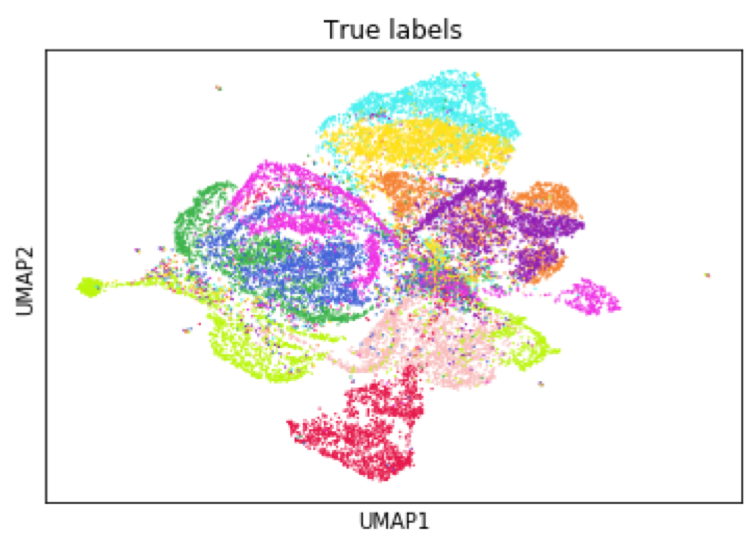
\includegraphics[width=\linewidth]{figs/notMNIST_labels.png} 
        %\caption{Price regulation} \label{fig:timing3}
    \end{subfigure}
    \begin{subfigure}[t]{0.15\textwidth}
    \centering
        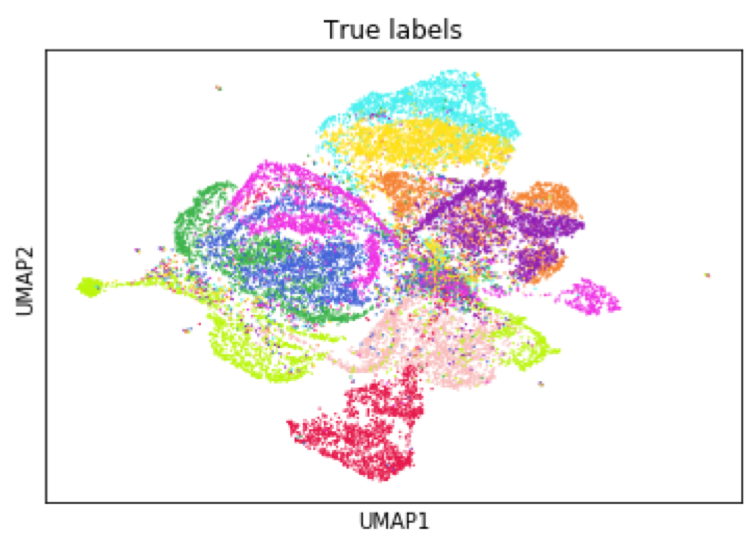
\includegraphics[width=\linewidth]{figs/notMNIST_labels.png} 
        %\caption{Price regulation} \label{fig:timing3}
    \end{subfigure}
    %\hfill
    \begin{subfigure}[t]{0.15\textwidth}
        \centering
        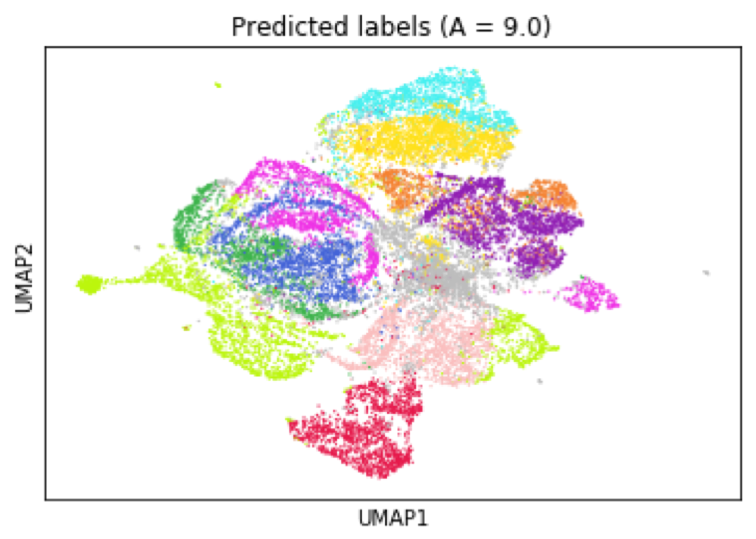
\includegraphics[width=\linewidth]{figs/notMNIST_preds_Aeq9.png} 
        %\caption{Competitors} \label{fig:timing2}
    \end{subfigure}
    \begin{subfigure}[t]{0.17\textwidth}
        \centering
        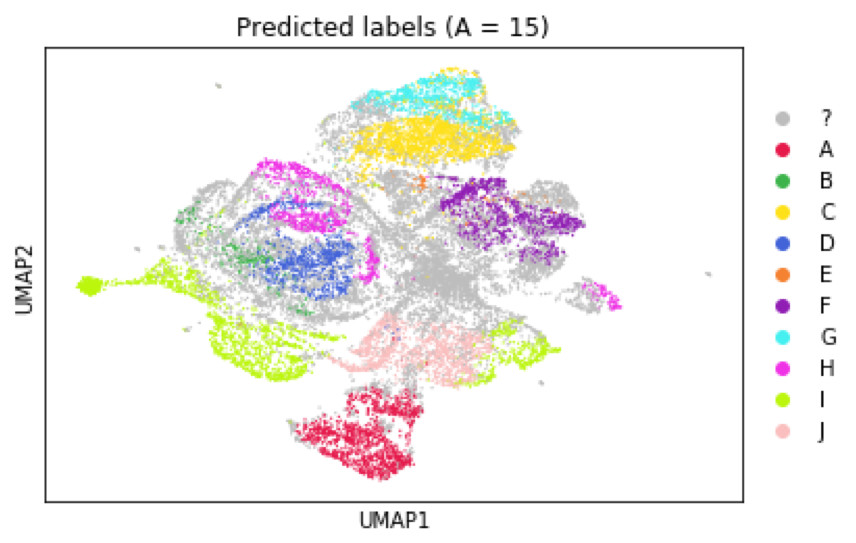
\includegraphics[width=\linewidth]{figs/notMNIST_preds_Aeq15.png} %\caption{Generic} \label{fig:timing1}
    \end{subfigure}
  \caption{Labels (left) and $\algname$ predictions (center \& right) on notMNIST}
  \label{fig:varyingparam}
\end{figure}





\begin{figure}
    \begin{subfigure}[t]{0.32\textwidth}
    \centering
        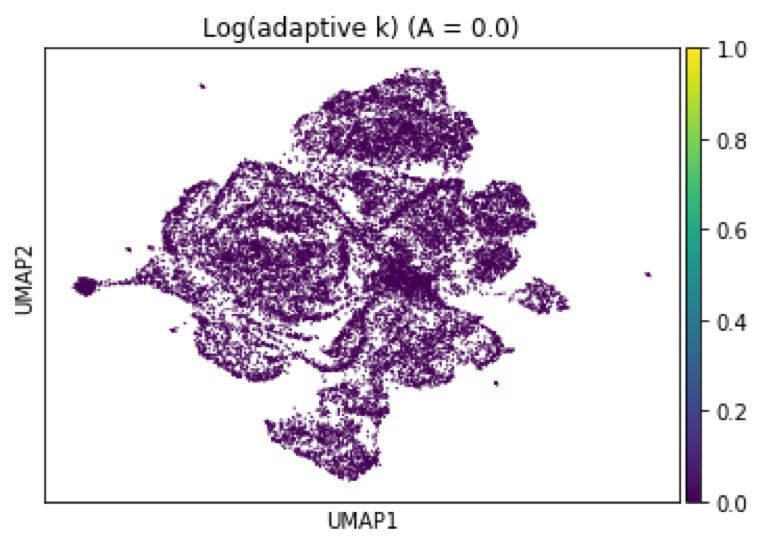
\includegraphics[width=\linewidth]{figs/notMNIST_logadaK_Aeq0.png} 
        %\caption{Price regulation} \label{fig:timing3}
    \end{subfigure}
    \begin{subfigure}[t]{0.32\textwidth}
        \centering
        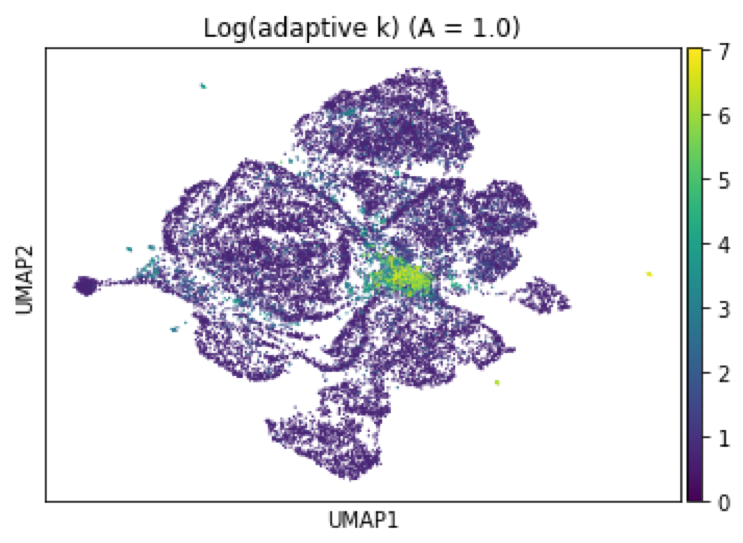
\includegraphics[width=\linewidth]{figs/notMNIST_logadaK_Aeq1.png} 
        %\caption{Competitors} \label{fig:timing2}
    \end{subfigure}
    \begin{subfigure}[t]{0.32\textwidth}
        \centering
        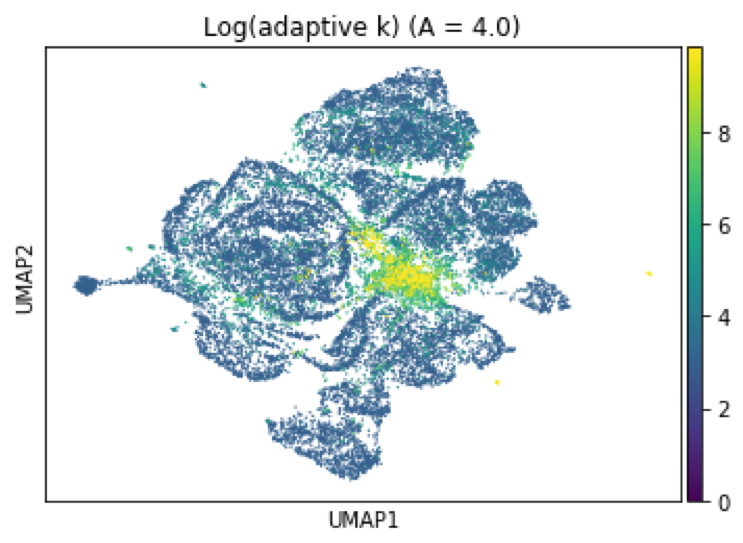
\includegraphics[width=\linewidth]{figs/notMNIST_logadaK_Aeq4.png} %\caption{Generic} \label{fig:timing1}
    \end{subfigure}
    \hfill
    
    \begin{subfigure}[t]{0.32\textwidth}
    \centering
        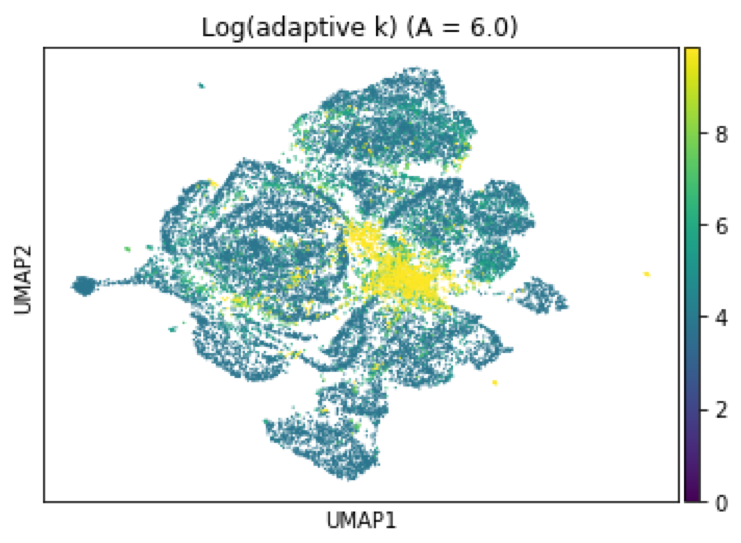
\includegraphics[width=\linewidth]{figs/notMNIST_logadaK_Aeq6.png} 
        %\caption{Price regulation} \label{fig:timing3}
    \end{subfigure}
    \begin{subfigure}[t]{0.32\textwidth}
        \centering
        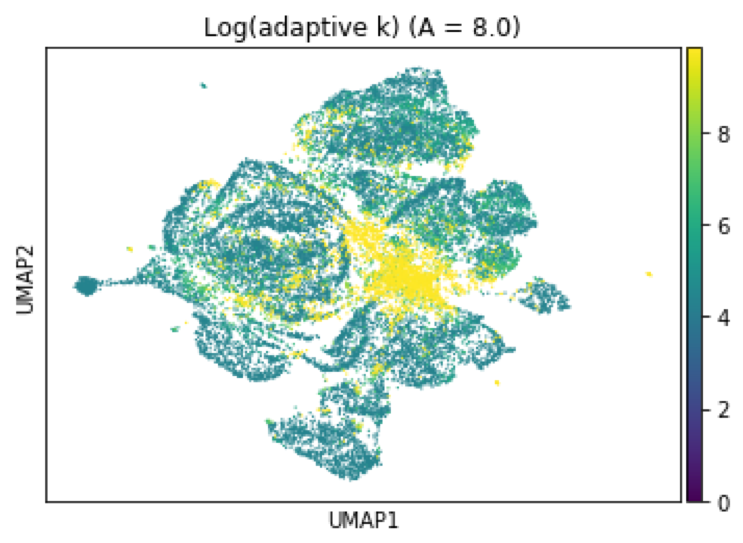
\includegraphics[width=\linewidth]{figs/notMNIST_logadaK_Aeq8.png} 
        %\caption{Competitors} \label{fig:timing2}
    \end{subfigure}
    \begin{subfigure}[t]{0.32\textwidth}
        \centering
        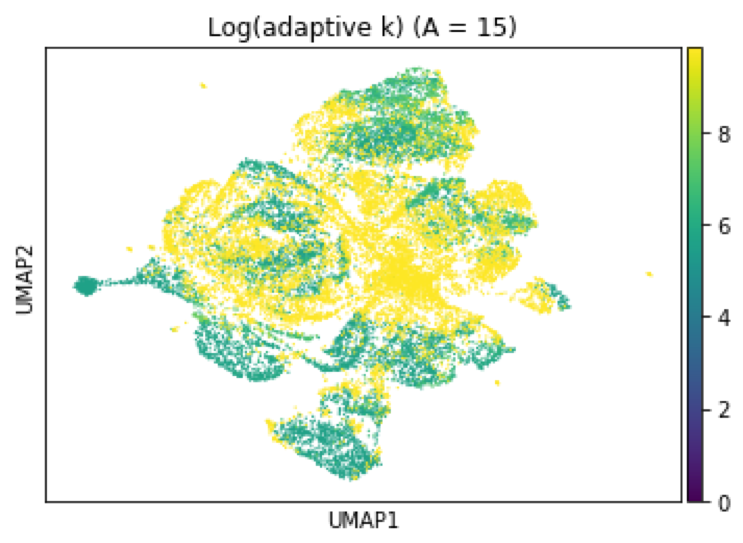
\includegraphics[width=\linewidth]{figs/notMNIST_logadaK_Aeq15.png} %\caption{Generic} \label{fig:timing1}
    \end{subfigure}
    \hfill
  \caption{$\algname$ neighborhood sizes on notMNIST, in increasing order of $A$, plotted on a log scale. Top left figure ($A = 0$) represents a $1$-NN classifier. Bottom right figure ($A = 15$) shows that many of the points' neighborhoods are maximally large, which can be compared to the right panel of Fig. \ref{fig:varyingparam}.}
  \label{fig:varyingadak}
\end{figure}


\subsection{$\algname$ is comparable to the best $k$-NN rule}

The discussions of Section \ref{sec:knn-comparison} prove that $\algname$ compares favorably to $k$-NN with any fixed $k$. We see this in practice as well (Fig. \ref{fig:aknnvsknn}). 

\begin{figure}
    \begin{subfigure}[t]{0.5\textwidth}
    \centering
        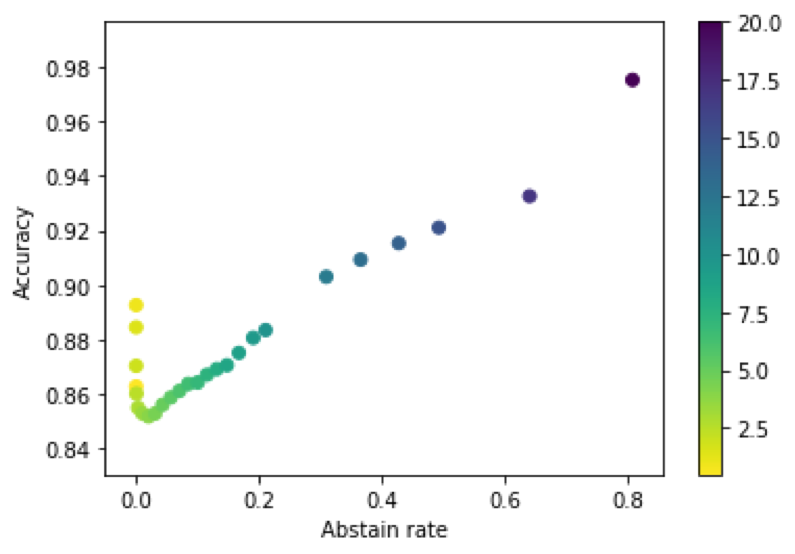
\includegraphics[width=\linewidth]{figs/notMNIST_accvsabst.png} 
        %\caption{Price regulation} \label{fig:timing3}
    \end{subfigure}
    \begin{subfigure}[t]{0.5\textwidth}
        \centering
        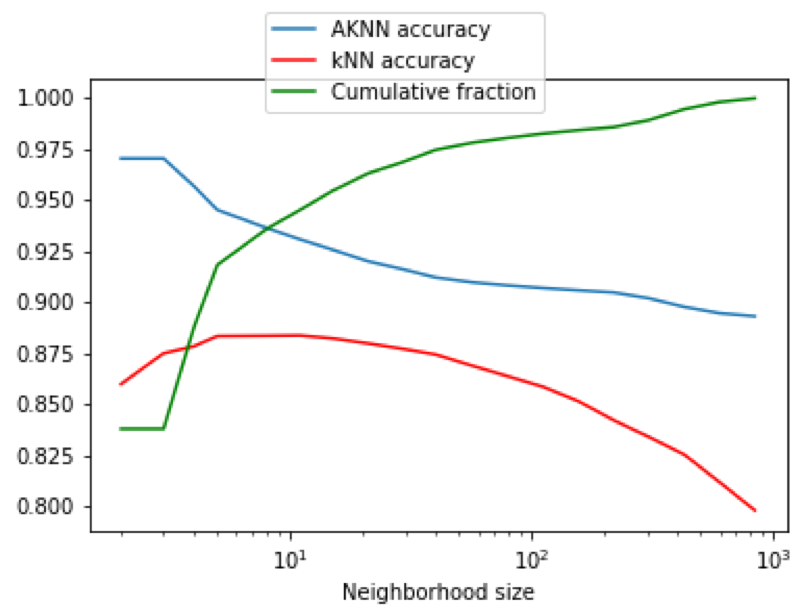
\includegraphics[width=\linewidth]{figs/notMNIST_aknnvsknn.png} 
        %\caption{Competitors} \label{fig:timing2}
    \end{subfigure}
    \hfill
  \caption{$\algname$ performance on notMNIST. \yoav{Akshay, Please expand the caption}}
  \label{fig:aknnvsknn}
\end{figure}















\bibliography{ref}
\bibliographystyle{alpha}



\appendix

\section{High-probability convergence}

In this section, we make a further assumption that allows us to strengthen \Cref{thm:general-error-bound}: 
the family of all balls in $(\X, d)$ has VC dimension $d_0 < \infty$. 
Given such a $d_0$ and parameter $\delta$, define $\kappa_{n, \delta} := d_0 \log n + \log (1/\delta)$. 
For $s \in \{ -1, +1 \}$, define the following quantities that depend on the algorithm's lone confidence parameter $\delta$:
\begin{align*}
\X^{s}_n (\delta)
:= \Bigg\{
x \in \supp(\mu) : s \eta(x) > 0 , \exists p_x > 0 \text{ s.t. } 
&s \eta(B(x,r_{p_x}(x))) \geq 2 c_2 \sqrt{\frac{ \kappa_{n, \delta} }{n p_x}}
\quad\text{and}\quad \\
&s \eta(B(x,r)) \geq 0 \quad\forall r \in (0, r_{p_x}(x)]
\Bigg\}
\end{align*}
where $c_2 = \max(2c_1, \frac{\varphi}{2} ) \sqrt{1 + c_0}$ for $\varphi := \frac{1}{2} (1 + \sqrt{5})$.
Also define 
$$ \partial_n (\delta) = \X \setminus (\X^+_{n,\delta} (\delta) \cup \X^-_{n,\delta}) $$
Then our main convergence rate result in this scenario shows that the measure of the effective boundary bounds the convergence of $\algname$.


\begin{theorem}\label{thm:fastrate2}
Let $\delta$ be the confidence parameter of the $\algname$ algorithm, and suppose \Cref{assump:VCallballs} holds with VC dimension $d_0$.
Then, with probability at least $1-\delta$ over the choice of training points,
\[ \pr_{X}(g_n(X) \neq g^*(X)) \ \leq \ \mu(\partial_n (\delta)) .\]
Here $g_n$ is the adaptive nearest neighbor classifier based on the $n$ training points and $g^*$ is the Bayes-optimal classifier. 
\end{theorem}

%\akshay{Is it worth showing that \Cref{thm:fastrate2} is tight, like the instance-dependent lower bounds of \cite{ChaudhuriDasgupta2014}?}


{\it To summarize, for convergence in expectation we bound the error by $\delta + \mu(\partial_n)$,
and for convergence with high probability we bound it by $\mu(\partial_n)$.}
So, in order to get explicit bounds in both settings, we need to figure out how $\mu(\partial_n)$ decays under natural assumptions. It would be nice if we could get something like 
\[\mu(\partial_n (\delta)) \leq \mathrm{poly}\left(\log(1/\delta), n\right),
\]
with hidden constant depending on the assumptions we make.
\akshay{The smoothness condition introduced in \cite{ChaudhuriDasgupta2014} may be relevant.}


% \subsection{Shay's comments}

% There are two natural settings we could consider: (i) convergence in expectation, and (ii) convergence with high probability.
% Convergence in expectation boils down to \Cref{thm:general-error-bound} in the previous section.
% For convergence with high probability we further assume that the VC dimension of the family of all balls is bounded. 
% Note that in this case we should also change the definition of $\Delta(n,k)$  in the algorithm so that it has the right dependence on the VC dimension. \akshay{It's already correct in the initial definition of the algorithm, but not consistent in the definitions of $\X^{\pm}_n$.} What we can prove in this case is \Cref{thm:fastrate} (stated in a subsection below), 
% which can also be phrased more similarly to \Cref{thm:general-error-bound}) as in \Cref{thm:fastrate2}.



\subsection{Proofs}

To prove \Cref{thm:fastrate2}, a relevant application of VC theory from \cite{ChaudhuriDasgupta2010} is useful:
\begin{lemma}[\cite{ChaudhuriDasgupta2010}, Lemma 16]
\label{lemma:points-in-balls-2}
There is an absolute constant $c_0$ such that the following holds. Let $\B$ be any class of measurable subsets of $\X$ of VC dimension $d_0$. Pick any $0 < \delta < 1$. Then with probability at least $1-\delta^2/2$ over the choice of $(x^{(1)}, y^{(1)}), \ldots, (x^{(n)}, y^{(n)})$, for all $B \in \B$ and for any integer $k$, we have
$$ \mu(B) \geq \frac{k}{n} + \frac{c_0}{n} \left( \kappa_{n, \delta} + \sqrt{k \kappa_{n, \delta}} \right)
\ \ \implies \ \ 
\mu_n(B) \geq \frac{k}{n} $$
\end{lemma}

\begin{proof}[Proof of \Cref{thm:fastrate2}]
Recall that we take the set $\B$ of all closed balls in $\X$ to have VC dimension at most $d_0$. 
By \Cref{lemma:points-in-balls-2} and \Cref{lemma:bias}, we have that with probability at least $1-\delta^2$, the following two properties hold for all $B \in \B$:
\begin{enumerate}
\item For any integer $k$, we have $\mu_n(B) \geq k/n$ whenever $n \mu(B) \geq k + c_0 \left( \kappa_{n, \delta} + \sqrt{k \kappa_{n, \delta}} \right)$
\item $|\bias_n(B) - \bias(B)| \leq \Delta(n, n \mu_n(B)) = c_1 \sqrt{\frac{\kappa_{n, \delta}}{n \mu_n(B)}}$
\end{enumerate}
Assume henceforth that these hold. Then it suffices to show that within this ``good" event, the adaptive-$k$ rule predicts correctly on $x \in \X^+_{n,\delta} \cup \X^-_{n,\delta}$ w.p. 1 under $\mu$. 

This argument is analogous to that of \Cref{lemma:good-sets}, with $\log (n/\delta)$ replaced by $\kappa_{n, \delta}$. We state the argument for $x \in \X^+_{n,\delta}$. Define $p(x) = p_x$ to be a function of $x$ as specified in the definition of $\X^+_{n,\delta}$, and set $k(x) = np(x) / (1 + c_0)$. We first observe that by definition of $p(x)$ and $c_2$, we have $c_2 \sqrt{\kappa_{n, \delta}/(n p(x))} \leq 1/2$, and thus $np(x) \geq 4 c_2^2 \kappa_{n, \delta} \geq \varphi^2 (1+c_0) \kappa_{n, \delta}$, so that $k(x) \geq \varphi^2 \kappa_{n, \delta}$. Therefore, $\frac{1}{c_0} (np(x) - k(x)) = k(x) = \left( \frac{1}{\varphi^2} + \frac{1}{\varphi} \right) k(x) \geq \kappa_{n, \delta} + \sqrt{ \kappa_{n, \delta} k(x) }$. Thus, by property 1, the ball $B = B(x, r_{p(x)} (x))$ has $\mu_n(B) \geq k(x)/n$. This means, in turn, that by property 2, 
\begin{align*}
\bias_n(B) &\geq \bias(B) - \Delta(n, k(x) ) 
\geq c_2 \sqrt{\frac{\kappa_{n, \delta}}{np}} - c_1 \sqrt{\frac{\kappa_{n, \delta}}{k(x)}} 
\geq 2c_1 \sqrt{\frac{\kappa_{n, \delta}}{k(x)}} - c_1 \sqrt{\frac{\kappa_{n, \delta}}{k(x)}} 
\geq \Delta(n, n \mu_n(B))
\end{align*}
So ball $B$ would trigger a prediction of $+1$.
At the same time, for any ball $B' = B(x, r)$ with $r < r_{p(x)} (x)$,
$$ \bias_n(B') \geq \bias(B') - \Delta(n, n \mu_n(B')) > -\Delta(n, n \mu_n(B')) $$
and thus no such ball will trigger a prediction of $-1$. Therefore, the algorithm's prediction at $x$ must be $+1$.

The argument for $x \in \X^-_{n,\delta}$ proceeds exactly symmetrically. 
\end{proof}

\section{Experimental Results}

\subsection{Datasets}

We test $\algname$ on the notMNIST dataset (\cite{notMNIST}), consisting of extracted glyphs of the letters A-J from publicly available fonts. We use the 18724 labeled examples from this set, preprocessed feature-wise to be in $[-\frac{1}{2}, \frac{1}{2}]$ using $x \mapsto \frac{x}{255} - \frac{1}{2}$.

We also test on the MNIST dataset. \yoav{I tried centering the bounding box, but it made the results worse, so I abandoned it. I am using unaltered Euclidean distance on the public MNIST data.}

We use $\algname$ on a challenging binary classification task of independent and continuing interest, involving single-cell gene expression data from different mouse organs collected by the Tabula Muris consortium (\cite{tabulamuris18}). The data are collected using representative protocols of the two currently dominant approaches to isolate and measure single cells: a ``plate"-based approach using microwells on a chip, and a ``droplet"-based approach manipulating cells within droplets using microfluidic technologies. Each approach has its own ill-understood set of technical biases, and discriminating between the two to identify these biases is currently of great interest.

\begin{figure}
\begin{center}
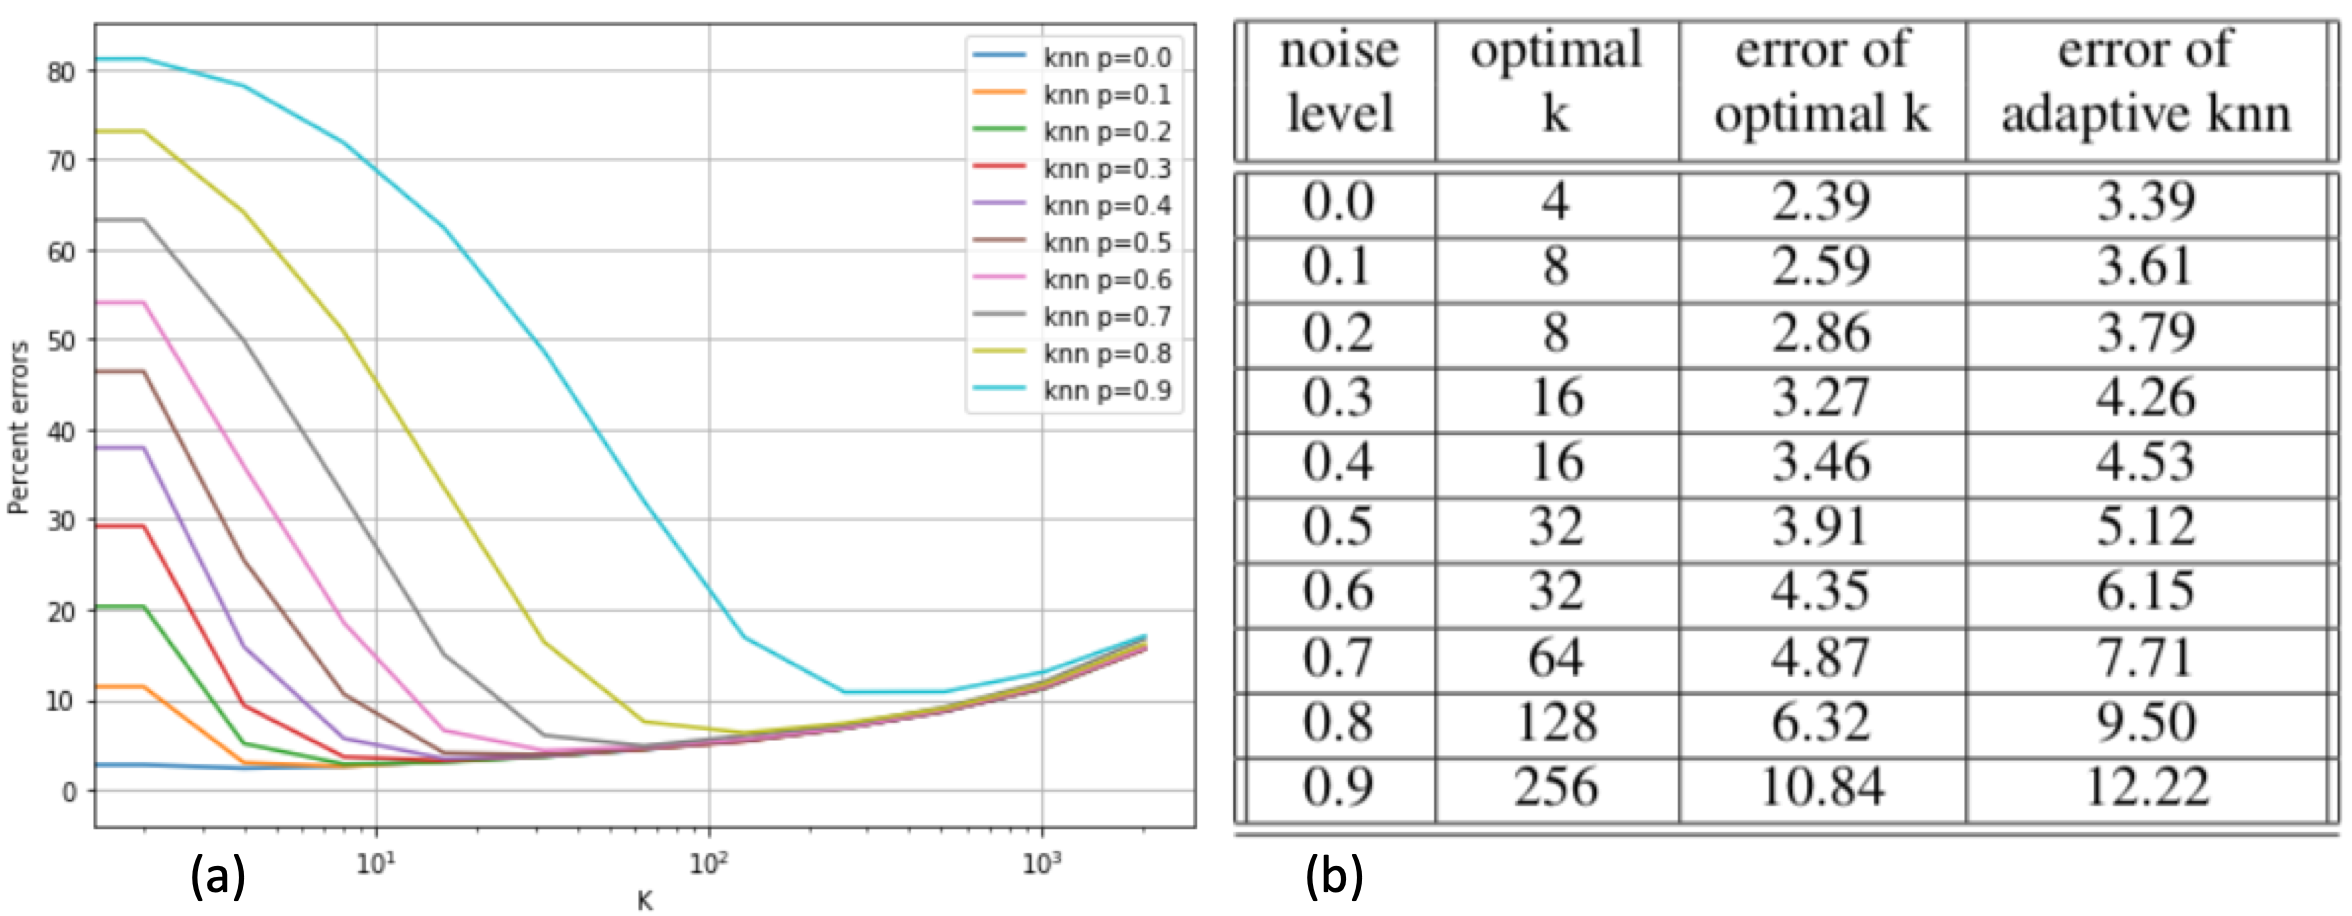
\includegraphics[width=6in]{figs/combined_figure.png}
\end{center}
\caption{Results from an experiment comparing the performance of k-NN on the MNIST data set for different noise levels $p$ and for different values of $k$. Note that the choice of $k$ has a large effect on the error, and that the larger the amount of noise $p$, the larger the value of $k$ needs to be.}
\label{fig:mnist}
\end{figure}


\end{document}

\iffalse
%A table comparing the performance of kNN, with the optimal choice of $k$ to that of Adaptive-kNN.

\begin{center}
 \begin{tabular}{||c | c | c | c||} 
 \hline
 noise & optimal & error of  & error of \\ 
 level &    k    & optimal k & adaptive knn \\  [0.5ex] 
 \hline\hline
 0.0 &    4 &  2.39 &  3.39 \\ \hline
 0.1 &    8 &  2.59 &  3.61 \\ \hline
 0.2 &    8 &  2.86 &  3.79 \\ \hline
 0.3 &   16 &  3.27 &  4.26 \\ \hline
 0.4 &   16 &  3.46 &  4.53 \\ \hline
 0.5 &   32 &  3.91 &  5.12 \\ \hline
 0.6 &   32 &  4.35 &  6.15 \\ \hline
 0.7 &   64 &  4.87 &  7.71 \\ \hline
 0.8 &  128 &  6.32 &  9.50 \\ \hline
 0.9 &  256 & 10.84 & 12.22 \\ \hline
 \hline
\end{tabular}
\end{center}
\fi
